\subsection{分次}

设 \(\Delta\) 是一个以加法记的交换幺半群。设 \(\phi_0\) 表示 X 到 \(\Delta\) 中的一个映射，并用 \(\phi\) 表示自由 magma M(X) 到 \(\Delta\) 中的扩张 \(\phi_0\) 的同态。对一切 \(\delta \in \Delta\) ，令 \(\operatorname{Lib}^{\delta}(X)\) 为 \(\operatorname{Lib}(X)\) 中以 M(X) 的子集 \(\phi^{-1}(\delta)\) 为基的子模。族 \((\operatorname{Lib}^{\delta}(X))_{\delta \in \Delta}\) 是代数 \(\operatorname{Lib}(X)\) 的一个分次，即

\begin{enumerate}
\def\labelenumi{(\arabic{enumi})}
\setcounter{enumi}{7}
\tightlist
\item
\end{enumerate}

\[
\operatorname{Lib} (\mathrm{X}) = \bigoplus_ {\delta \in \Delta} \operatorname{Lib} ^ {\delta} (\mathrm{X})\tag{8}
\]

\[
\operatorname{Lib} ^ {\delta} (\mathrm{X}). \operatorname{Lib} ^ {\delta^ {\prime}} (\mathrm{X}) \subset \operatorname{Lib} ^ {\delta + \delta^ {\prime}} (\mathrm{X}) \quad \text { for } \delta , \delta^ {\prime} \text { in } \Delta\tag{9}
\]

(《代数》， 第 III 章， § 3， no. 1， 例 3)。

引理 1. 定义 1 中的理想 \(\mathfrak{a}\) 是分次的。

设 \(a, b\) 属于 \(\operatorname{Lib}(\mathbf{X})\) ，令 \(\mathbf{B}(a, b) = a.b + b.a\) 。公式

\begin{enumerate}
\def\labelenumi{(\arabic{enumi})}
\setcounter{enumi}{9}
\tightlist
\item
\end{enumerate}

\[
\mathrm{B} (a, b) = \mathrm{Q} (a + b) - \mathrm{Q} (a) - \mathrm{Q} (b)\tag{10}
\]

\[
Q \left(\lambda_ {1}. w _ {1} + \dots + \lambda_ {n}. w _ {n}\right) = \sum_ {i} \lambda_ {i} ^ {2} Q \left(w _ {i}\right) + \sum_ {i <   j} \lambda_ {i} \lambda_ {j} B \left(w _ {i}, w _ {j}\right)\tag{11}
\]

对 M(X) 中的 \(w_1, \ldots, w_n\) 与 K 中的 \(\lambda_1, \ldots, \lambda_n\) 表明，族 \((\mathbf{Q}(a))_{a \in \mathrm{Lib}(\mathbf{X})}\) 与 \((\mathbf{Q}(w), \mathbf{B}(w, w'))_{w, w' \in \mathrm{M}(\mathbf{X})}\) 生成 Lib(X) 的同一个子模。由于 J 是三线性的，理想 a 由齐次元素 \(\mathbf{Q}(w), \mathbf{B}(w, w')\) 与 \(\mathbf{J}(w, w', w'')\) 生成，其中 \(w, w', w''\) 属于 M(X)，因而它是分次的 (《代数》， 第 III 章， § 3， no. 3， 命题 1)。

给李代数 \(\mathrm{L}(\mathbf{X}) = \mathrm{Lib}(\mathbf{X}) / a\) 赋予商分次。\(\mathrm{L}(\mathbf{X})\) 的 \(\delta\) 次齐次分量记作 \(\mathrm{L}^{\delta}(\mathbf{X})\) ；它是 \(\mathrm{L}(\mathbf{X})\) 中由元素 \(w \in \mathrm{M}(\mathbf{X})\) （它们满足 \(\phi(w) = \delta\) ）的像生成的子模。

我们将特别用到以下两种情形：

\begin{enumerate}
\def\labelenumi{(\alph{enumi})}
\tightlist
\item
  全分次：我们取 \(\Delta = \mathbf{N}\) ，\(\phi_0(x) = 1\) （对一切 \(x\in \mathbf{X}\) ），从而得到 \(\phi (w) = l(w)\) ，其中 \(w\) 属于 \(\mathrm{M}(\mathrm{X})\) 。K-模 \(\mathrm{L}^n (\mathrm{X})\) 由长度为 \(n\) 、属于 \(\mathrm{M}(\mathrm{X})\) 的元素的像生成，我们称这些元素为 \(n\) 次交错元。后面将会看到，模 \(\mathrm{L}^n (\mathrm{X})\) 是自由的，并且具有由 \(n\) 次交错元组成的一个基 (no. 11， 定理 1)。于是 \(\mathrm{L}(\mathrm{X}) = \bigoplus_{n\geq 1}\mathrm{L}^n (\mathrm{X})\) ，并且 \(\mathrm{L}^1 (\mathrm{X})\) 以 X 为基 (no. 2， 命题 1 的推论 1)。按照 \(\mathrm{M}(\mathrm{X})\) 的构造，
\end{enumerate}

\[
\mathrm{L} ^ {n} (\mathrm{X}) = \sum_ {p = 1} ^ {n - 1} [ \mathrm{L} ^ {p} (\mathrm{X}), \mathrm{L} ^ {n - p} (\mathrm{X}) ]\tag{12}
\]

特别地

\[
[ \mathrm{L} ^ {m} (\mathrm{X}), \mathrm{L} ^ {n} (\mathrm{X}) ] \subset \mathrm{L} ^ {m + n} (\mathrm{X}).\tag{13}
\]

\begin{enumerate}
\def\labelenumi{(\alph{enumi})}
\setcounter{enumi}{1}
\tightlist
\item
  多重分次：我们取 \(\Delta\) 为在 X 上构造的自由交换幺半群 \(\mathbf{N}^{(\mathbf{X})}\) 。映射 \(\phi_0\) 把 X 映到 \(\Delta\) 中，由 \((\phi_0(x))(x') = \delta_{xx'}\) 定义，其中 \(\delta_{xx'}\) 是 Kronecker 符号。对 \(w \in M(X)\) 与 \(x \in X\) ，整数 \((\phi(w))(x)\) 是“字母 \(x\) 在 \(w\) 中出现的次数”。设 \(\alpha\) 属于 \(\mathbf{N}^{(\mathbf{X})}\) ，我们记 \(|\alpha| = \sum_{x \in X} \alpha(x)\) ，从而 \(|\phi(w)| = l(w)\) （对 M(X) 中的一切 \(w\) ）。由此可得
\end{enumerate}

\[
\mathbf {L} ^ {n} (\mathbf {X}) = \bigoplus_ {| \alpha | = n} \mathbf {L} ^ {\alpha} (\mathbf {X});\tag{14}
\]

显然

\[
[ \mathrm{L} ^ {\alpha} (\mathrm{X}), \mathrm{L} ^ {\beta} (\mathrm{X}) ] \subset \mathrm{L} ^ {\alpha + \beta} (\mathrm{X}) \quad \text { for } \alpha , \beta \text { in } \mathbf {N} ^ {(\mathrm{X})}.\tag{15}
\]

命题 4. 设 \(S\) 是 \(X\) 的一个子集。若将 \(\mathbf{N}^{(\mathbb{S})}\) 与它在 \(\mathbf{N}^{(\mathbf{X})}\) 中的典范像等同 (《代数》， 第 I 章， § 7， no. 7)，则 \(L(S) = \sum_{\alpha \in \mathbf{N}^{(\mathbb{S})}} L^{\alpha}(X)\) 。此外，对一切 \(\alpha \in \mathbf{N}^{(\mathbb{S})}\) ， \(\alpha\) 次齐次分量（在 \(L(S)\) 上的多重分次之下）等于 \(L^{\alpha}(X)\) 。

 设 \(\alpha \in \mathbf{N}^{(S)}\) 。模 \(\mathrm{L}^{\alpha}(\mathrm{S})\) 由 \(\mathrm{L}(\mathrm{X})\) 中的像生成，即元素 \(w\) （属于 \(\mathrm{M}(\mathrm{S})\) 且满足 \(\phi(w) = \alpha\) ）的像，也就是说 (《代数》， § 7， no. 9， 公式 (23) 与 (24))，它是 \(w\) 组成的集合，其中元素属于 \(\mathrm{M}(\mathrm{X})\) 且满足 \(\phi(w) = \alpha\) 。由此得 \(\mathrm{L}^{\alpha}(\mathrm{S}) = \mathrm{L}^{\alpha}(\mathrm{X})\) 。命题由这一点以及关系式 \(\mathrm{L}(\mathrm{S}) = \sum_{\alpha \in \mathbf{N}^{(S)}}\mathrm{L}^{\alpha}(\mathrm{S})\) 得证。

推论. 对每个子集族 \((\mathbf{S}_i)_{i\in I}\) （子集取自 \(\mathbf{X}\) ），

\[
\mathrm{L} \left(\bigcap_ {i \in I} S _ {i}\right) = \bigcap_ {i \in I} \mathrm{L} (S _ {i}).\tag{16}
\]

这由命题 4 以及显然的公式

\[
\mathbf {N} ^ {(S)} = \bigcap_ {i \in I} \mathbf {N} ^ {(S _ {i})}\tag{17}
\]

得出，其中我们已记 \(S = \bigcap_{i \in I} S_i\) 。

\subsection{下中心列}

命题 5. 设 \(\mathfrak{g}\) 是一个李代数， \(\mathrm{P}\) 是 \(\mathfrak{g}\) 的一个子模。我们把子模 \(\mathrm{P}_n\) 定义在 \(\mathfrak{g}\) 中，公式为 \(\mathrm{P}_1 = \mathrm{P}\) 以及 \(\mathrm{P}_{n+1} = [\mathrm{P},\mathrm{P}_n]\) （对每个 \(n\geqslant 1\) ）。那么

\begin{enumerate}
\def\labelenumi{(\arabic{enumi})}
\setcounter{enumi}{17}
\tightlist
\item
\end{enumerate}

\[
[ \mathrm{P} _ {m}, \mathrm{P} _ {n} ] \subset \mathrm{P} _ {m + n},\tag{18}
\]

\[
\mathrm{P} _ {n} = \sum_ {p = 1} ^ {n - 1} \left[ \mathrm{P} _ {p}, \mathrm{P} _ {n - p} \right] for n \geqslant 2.\tag{19}
\]

我们对 \(m\) 作归纳来证明 (18)。情形 \(m = 1\) 是显然的。由 Jacobi 恒等式，

\[
[ [ \mathrm{P}, \mathrm{P} _ {m} ], \mathrm{P} _ {n} ] \subset [ \mathrm{P} _ {m}, [ \mathrm{P}, \mathrm{P} _ {n} ] ] + [ \mathrm{P}, [ \mathrm{P} _ {m}, \mathrm{P} _ {n} ] ],
\]

即

\[
[ \mathrm{P} _ {m + 1}, \mathrm{P} _ {n} ] \subset [ \mathrm{P} _ {m}, \mathrm{P} _ {n + 1} ] + [ \mathrm{P}, [ \mathrm{P} _ {m}, \mathrm{P} _ {n} ] ].
\]

归纳假设表明 \([\mathbf{P}_m, \mathbf{P}_{n+1}] \subset \mathbf{P}_{m+n+1}\) 且 \([\mathbf{P}_m, \mathbf{P}_n] \subset \mathbf{P}_{m+n}\) ，从而

\[
[ \mathrm{P} _ {m + 1}, \mathrm{P} _ {n} ] \subset \mathrm{P} _ {m + n + 1} + [ \mathrm{P}, \mathrm{P} _ {m + n} ] = \mathrm{P} _ {m + n + 1}.
\]

由公式 (18)， \(\mathrm{P}_n\supset \sum_{p = 1}^{n - 1}[\mathrm{P}_p,\mathrm{P}_{n - p}]\supset [\mathrm{P}_1,\mathrm{P}_{n - 1}] = \mathrm{P}_n\) ，由此得 (19)。

当取 \(\mathbf{P} = \mathfrak{g}\) 时，序列 \((\mathrm{P}_n)\) 就是下中心列 \((\mathcal{C}^n\mathfrak{g})\) （对 \(\mathfrak{g}\) 而言）(第 I 章， § 1， no. 5)。于是：

命题 6. 设 g 是一个李代数， \((\mathcal{C}^{n}\mathfrak{g})_{n\geqslant 1}\) 是 g 的下中心列。那么

\[
[ \mathcal {C} ^ {m} \mathfrak {g}, \mathcal {C} ^ {n} \mathfrak {g} ] \subset \mathcal {C} ^ {m + n} \mathfrak {g} \quad for m \geqslant 1 and n \geqslant 1.
\]

推广第 I 章 § 4 no. 1 中的定义 1，我们称李代数 g 是幂零的，如果 \(\mathcal{C}^{n}\mathfrak{g} = \{0\}\) （对充分大的 \(n\) ）。幂零李代数 g 的幂零类是最小的整数 \(n\) ，它使得 \(\mathcal{C}^{n + 1}\mathfrak{g} = \{0\}\) 成立。

命题 7. 设 X 是一个集合，n 是一个 ≥1 的整数。

\begin{enumerate}
\def\labelenumi{(\alph{enumi})}
\item
  \(\mathrm{L}^{n+1}(\mathrm{X}) = [\mathrm{L}^{1}(\mathrm{X}), \mathrm{L}^{n}(\mathrm{X})]\) 。
\item
  模 \(L^{n}(X)\) 由形如 \([x_{1}, [x_{2}, \ldots, [x_{n-1}, x_{n}] \ldots]]\) 的元素生成，其中 \((x_{1}, \ldots, x_{n})\) 取遍由 X 的 n 个元素组成的序列的集合。
\item
  L(X) 的下中心列由 \(\mathcal{C}^n (\mathrm{L}(\mathrm{X})) = \sum_{p\geqslant n}\mathrm{L}^p (\mathrm{X})\) 给出
\item
  我们取 \(\mathfrak{g} = \mathrm{L}(\mathrm{X})\) 与 \(\mathrm{P} = \mathrm{L}^{1}(\mathrm{X})\) 应用命题 5。对 \(n\) 作归纳，由 (12) (no. 6) 与 (19) 推出等式 \(\mathrm{P}_{n} = \mathrm{L}^{n}(\mathrm{X})\) 。所欲证的关系式于是等价于定义 \([\mathrm{P}, \mathrm{P}_{n}] = \mathrm{P}_{n + 1}\) 。
\item
  这由 (a) 对 \(n\) 作归纳得到。
\item
  设 \(\mathfrak{g} = \mathrm{L}(\mathrm{X})\) 与 \(\mathfrak{g}_{n} = \sum_{p\geqslant n}\mathrm{L}^{p}(\mathrm{X})\) 。那么 \(\mathfrak{g} = \mathfrak{g}_1\) ，并且 no. 6 的公式 (13) 蕴涵 \([\mathfrak{g}_{n},\mathfrak{g}_{m}]\subset \mathfrak{g}_{n + m}\) ，特别地有 \([\mathfrak{g},\mathfrak{g}_n]\subset \mathfrak{g}_{n + 1}\) 。对 \(n,\mathcal{C}^{n}\mathfrak{g}\subset \mathfrak{g}_{n}\) 作归纳。另一方面，由 (a) 我们归纳地导出 \(\mathrm{L}^{n}(\mathrm{X})\subset \mathcal{C}^{n}\mathfrak{g}\) （对 \(n\) 归纳）。由于 \(\mathcal{C}^{n}\mathfrak{g}\) 是 \(\mathfrak{g}\) 的一个理想，关系式 \(\mathrm{L}^p (\mathrm{X})\subset \mathcal{C}^{n}\mathfrak{g}\) 蕴涵
\end{enumerate}

\[
\mathrm{L} ^ {p + 1} (\mathrm{X}) = [ \mathrm{L} ^ {1} (\mathrm{X}), \mathrm{L} ^ {p} (\mathrm{X}) ] \subset \mathcal {C} ^ {n} \mathfrak {g}
\]

这由 (a) 得出。因此有 \(\mathbf{L}^p (\mathbf{X})\subset \mathcal{C}^{n}\mathfrak{g}\) （对 \(p\geqslant n\) ），从而 \(\mathfrak{g}_n\subset \mathcal{C}^{n}\mathfrak{g}\)

推论. 设 \(\mathfrak{g}\) 是一个李代数， \((x_{i})_{i\in I}\) 是 \(\mathfrak{g}\) 的一个生成族。下中心列的第 \(n\) 项 \(\mathcal{C}^{n}\mathfrak{g}\) （对 \(\mathfrak{g}\) 而言）是由迭代括号 \([x_{i_1}, [x_{i_2}, \ldots, [x_{i_{p-1}}, x_{i_p}] \ldots]]\) 生成的模，其中 \(p \geqslant n\) ，且 \(i_1, \ldots, i_p\) 属于 I。

设 \(f\) 是 L(I) 到 g 中的同态，使得 \(f(i) = x_i\) （对一切 \(i \in I\) ）。由于 \((x_i)_{i \in I}\) 生成 g，有 g = f(L(I))，从而由第 I 章 § 1 no. 5 的命题 4 得 \(\mathcal{C}^{\bullet}g = f(\mathcal{C}^{\bullet}(L(I)))\) 。推论于是由命题 7 的断言 (b) 与 (c) 得出。

\subsection{自由李代数的导子}

命题 8. 设 X 是一个集合，M 是一个 L(X)-模，d 是 X 到 M 中的一个映射。存在且仅存在一个 L(X) 到 M 中的线性映射 D，它扩张 d 并且满足关系式：

\[
\mathrm{D} ([ a, a ^ {\prime} ]) = a. \mathrm{D} (a ^ {\prime}) - a ^ {\prime}. \mathrm{D} (a) \quad for a, a ^ {\prime} in \mathrm{L} (\mathrm{X}).\tag{20}
\]

我们借助括号定义一个以模 M × L(X) 为基础模的李代数 g

\[
[ (m, a), (m ^ {\prime}, a ^ {\prime}) ] = (a. m ^ {\prime} - a ^ {\prime}. m, [ a, a ^ {\prime} ]),\tag{21}
\]

其中 \(a, a'\) 属于 \(\mathrm{L}(\mathrm{X})\) 且 \(m, m'\) 属于 \(\mathbf{M}\) (第 I 章， § 1， no. 8)。设 \(f\) 是 \(\mathrm{L}(\mathrm{X})\) 到 \(\mathfrak{g}\) 中的同态，使得 \(f(x) = (d(x), x)\) 对一切 \(x\) （属于 \(\mathbf{X}\) ）成立；令 \(f(a) = (\mathrm{D}(a), u(a))\) （\(a\) 取遍 \(\mathrm{L}(\mathrm{X})\) ）。由公式 (21)， \(u\) 是 \(\mathrm{L}(\mathrm{X})\) 到其自身的同态；由于 \(u(x) = x\) 对每个 \(x\) （属于 \(\mathbf{X}\) ）成立，故 \(u(a) = a\) 对一切 \(a\) （属于 \(\mathrm{L}(\mathrm{X})\) ）成立，从而

\[
f (a) = (\mathrm{D} (a), a).\tag{22}
\]

于是由 (21) 与 (22)，关系式 (20) 可由 \(f([a, a']) = [f(a), f(a')]\) 得出。

反之，设 \(D'\) 是 \(\mathrm{L}(\mathrm{X})\) 到 M 中的一个映射，它满足与 (20) 类似的关系式 \((20')\) 并且扩张 d。令 \(f'(a) = (\mathrm{D}'(a), a)\) （对每个 \(a \in \mathrm{L}(\mathrm{X})\) ）；由 \((20')\) 与 \((21)\) ， \(f'\) 是 \(\mathrm{L}(\mathrm{X})\) 到 g 中的一个同态，并且在 X 上与 f 一致，从而 \(f' = f\) 且 \(D' = D\) 。

推论. \(\mathbf{X}\) 到 \(\mathrm{L}(\mathbf{X})\) 中的每个映射都可以唯一地扩张为 \(\mathrm{L}(\mathbf{X})\) 的一个导子。

当 M 取伴随表示下的 L(X) 时，关系式 (20) 表示 D 是一个导子。

\subsection{消元定理}

命题 9. 设 \(\mathbf{S}_1\) 与 \(\mathbf{S}_2\) 是两个不相交的集合， \(d\) 是 \(\mathbf{S}_1 \times \mathbf{S}_2\) 到 \(\mathrm{L}(\mathbf{S}_2)\) 中的一个映射。设 \(\mathfrak{g}\) 是 \(\mathrm{L}(\mathbf{S}_1 \cup \mathbf{S}_2)\) 对由元素 \([s_1, s_2] - d(s_1, s_2)\) （满足 \(s_1 \in \mathbf{S}_1\) 与 \(s_2 \in \mathbf{S}_2\) ）生成的理想所作的商李代数；设 \(\psi\) 是 \(\mathrm{L}(\mathbf{S}_1 \cup \mathbf{S}_2)\) 到 \(\mathfrak{g}\) 上的典范映射。

\begin{enumerate}
\def\labelenumi{(\alph{enumi})}
\item
  对 \(i = 1,2\) ， \(\phi_{i}\) （即 \(\psi\) 在 \(S_{i}\) 上的限制）可以扩张为 \(\mathbf{L}(S_i)\) 到一个子代数 \(\mathfrak{a}_i\) （包含于 \(\mathfrak{g}\) ）上的同构。
\item
  \(\mathfrak{g} = \mathfrak{a}_1 + \mathfrak{a}_2, \mathfrak{a}_1 \cap \mathfrak{a}_2 = \{0\}\) ，并且 \(\mathfrak{a}_2\) 是 \(\mathfrak{g}\) 的一个理想。
\end{enumerate}

对 \(i = 1,2\) ，用 \(\psi_{i}\) 表示 \(\mathbf{L}(\mathbf{S}_i)\) 到 \(\mathfrak{g}\) 中的扩张 \(\phi_i\) 的同态，并用 \(\mathfrak{a}_i\) 表示它的像。显然 \(\phi_i(\mathbf{S}_i)\) 生成 \(\mathfrak{a}_i\) 。

设 \(s_1 \in S_1\) ；我们记 \(D = \operatorname{ad} \phi_1(s_1)\) 。 \(D\) 是 \(g\) 的一个导子，它把 \(\phi_2(S_2)\) 映到 \(a_2\) 之中，依照关系式

\[
[ \phi_ {1} (s _ {1}), \phi_ {2} (s _ {2}) ] = \psi_ {2} (d (s _ {1}, s _ {2})) \quad \text { for } s _ {2} \in S _ {2};
\]

由于 \(\mathfrak{a}_2\) 作为 \(\mathfrak{g}\) 的子代数由 \(\phi_2(S_2)\) 生成，因此 \(D(\mathfrak{a}_2) \subset \mathfrak{a}_2\) 。由那些 \(x \in \mathfrak{g}\) （它们使 ad \(x\) 保持 \(\mathfrak{a}_2\) 不变）组成的集合是 \(\mathfrak{g}\) 的一个李子代数，由上所述它包含 \(\phi_1(S_1)\) ，从而也包含 \(\mathfrak{a}_1\) 。因此

\[
\left[ \mathfrak {a} _ {1}, \mathfrak {a} _ {2} \right] \subset \mathfrak {a} _ {2}.\tag{23}
\]

因此 \(a_1 + a_2\) 是 \(g\) 的一个李子代数，并且由于它包含生成集 \(\phi_1(S_1) \cup \phi_2(S_2)\) ，

\[
a _ {1} + a _ {2} = g.\tag{24}
\]

对一切 \(s_1 \in S_1\) ，存在导子 \(D_{s_1}\) （\(L(S_2)\) 上的），使得

\[
\mathrm{D} _ {s _ {1}} (s _ {2}) = d (s _ {1}, s _ {2})
\]

对一切 \(s_2\) （属于 \(S_2\) ）成立 (no. 8， 命题 8 的推论)。映射 \(s_1 \mapsto D_{s_1}\) 可以扩张为一个同态 \(D\) （从 \(L(S_1)\) 到 \(L(S_2)\) 的导子李代数中）。设 \(\mathfrak{h}\) 是 \(L(S_1)\) 与 \(L(S_2)\) 的对应于 \(D\) 的半直积 (第 I 章， § 1， no. 8)。作为模， \(\mathfrak{h}\) 等于 \(L(S_1) \times L(S_2)\) ，特别地

\[
[ (s _ {1}, 0), (0, s _ {2}) ] = (0, d (s _ {1}, s _ {2}))\tag{25}
\]

其中 \(s_{1} \in S_{1}\) 与 \(s_{2} \in S_{2}\) 。

由 (25) 我们推出存在一个同态 \(f\) （从 \(\mathfrak{g}\) 到 \(\mathfrak{h}\) 中），使得 \(f(\phi_1(s_1)) = (s_1, 0)\) ，并且 \(f(\phi_2(s_2)) = (0, s_2)\) （对 \(s_1 \in S_1\) 与 \(s_2 \in S_2\) ）。我们立即推出关系式

\[
f (\psi_ {1} (a _ {1}) + \psi_ {2} (a _ {2})) = (a _ {1}, a _ {2})\tag{26}
\]

其中 \(a_1 \in \mathrm{L}(\mathrm{S}_1)\) 与 \(a_2 \in \mathrm{L}(\mathrm{S}_2)\) 。

关系式 (26) 表明 \(\psi_{1}\) 与 \(\psi_{2}\) 都是单射，并且 \(a_{1} \cap a_{2} = \{0\}\) 。于是公式 (23) 与 (24) 蕴涵本命题。

命题 10 (消元定理). 设 X 是一个集合，S 是 X 的一个子集，T 是由这样的序列 \((s_1, \ldots, s_n, x)\) 组成的集合：\(n \geqslant 0\) ， \(s_1, \ldots, s_n\) 属于 S 且 \(x\) 属于 \(\mathbf{X} - \mathbf{S}\) 。

\begin{enumerate}
\def\labelenumi{(\alph{enumi})}
\item
  模 \(\mathbf{L}(\mathbf{X})\) 是子代数 \(\mathbf{L}(\mathbf{S})\) （\(\mathbf{L}(\mathbf{X})\) 中的）与理想 \(\mathfrak{a}\) （\(\mathbf{L}(\mathbf{X})\) 中由 \(\mathbf{X} - \mathbf{S}\) 生成的）的直和。
\item
  存在一个李代数同构 \(\phi\) （从 L(T) 到 \(\mathfrak{a}\) 上），它把 \((s_1, \ldots, s_n, x)\) 映为 (ad \(s_1 \circ \cdots \circ\) ad \(s_n\) ) ( \(x\) )。
\end{enumerate}

设 \(g\) 是按命题 9 的方式构造的李代数，给定

\[
\mathrm{S} _ {1} = \mathrm{S}, \quad \mathrm{S} _ {2} = \mathrm{T}, \quad d (s, t) = (s, s _ {1}, \dots , s _ {n}, x) \in \mathrm{T} \subset \mathrm{L} (\mathrm{T})
\]

其中 \(t = (s_1, \ldots, s_n, x)\) 属于 \(T\) 且 \(s \in S_1\) 。我们把 \(L(S)\) 与 \(L(T)\) 和它们在 \(g\) 中的典范像等同 (命题 9 (a))。

设 \(\psi\) 是映射 \((s_1, \ldots, s_n, x) \mapsto (\operatorname{ad} s_1 \circ \cdots \circ \operatorname{ad} s_n)(x)\) （从 T 到 \(\mathrm{L}(\mathbf{X})\) 中）。显然 \(\psi(d(s, t)) = [s, \psi(t)]\) （对 \(s \in S\) 与 \(t \in T\) ），因而存在一个同态 \(\alpha: g \to L(X)\) ，它在 \(S\) 上的限制是恒同映射，而在 \(T\) 上的限制是 \(\psi\) 。而 \(X - S \subset T\) ，从而存在一个同态 \(\beta: L(X) \to g\) ，它在 \(X = S \cup (X - S)\) 上的限制是恒同映射。

我们证明 \(\alpha\) 是一个同构，而 \(\beta\) 是其逆同构。由于 \(\psi(x) = x\) 对每个 \(x\) （属于 \(\mathbf{X} - \mathbf{S}\) ）成立，我们看出 \(\alpha \circ \beta\) 在 \(\mathbf{X}\) 上与恒同映射一致，从而 \(\alpha \circ \beta = \mathrm{Id}_{\mathrm{L}(\mathbf{X})}\) 。另一方面，按构造， \([s, t] = d(s, t)\) 属于 \(\mathfrak{g}\) （对 \(s \in \mathbb{S}\) 与 \(t \in \mathbb{T}\) ）；由此推出 \(t = (s_1, \ldots, s_n, x)\) 在 \(\mathfrak{g}\) 中等于 \((\operatorname{ad} s_1 \circ \cdots \circ \operatorname{ad} s_n)(x)\) ，从而 \(t = \beta(\alpha(t))\) 。由于 \(\beta(\alpha(s)) = s\) （对 \(s \in \mathbb{S}\) ），并且 \(\mathbb{S} \cup \mathbb{T}\) 生成 \(\mathfrak{g}, \beta \circ \alpha = \mathrm{Id}_{\mathfrak{g}}\) 。

由于 \(\alpha\) 是 \(g\) 到 \(L(X)\) 上的一个同构，命题 9 表明 \(\alpha\) 在 \(\mathrm{L(T)}\) 上的限制是一个同构 \(\phi\) ，它把 \(\mathrm{L(T)}\) 映到一个理想 \(\mathfrak{b}\) （\(\mathrm{L(X)}\) 中的）上，使得模 \(\mathrm{L(X)}\) 是 \(\mathrm{L(S)}\) 与 \(\mathfrak{b}\) 的直和。显然

\[
\phi (s _ {1}, \dots , s _ {n}, x) = (\operatorname{ad} s _ {1} \circ \dots \circ \operatorname{ad} s _ {n}) (x)
\]

其中 T 中的 \((s_1, \ldots, s_n, x)\) 。

因此 \(\phi(T) \subset \mathfrak{a}\) ，而 \(\mathfrak{b} \subset \mathfrak{a}\) ，因为 \(\phi(T)\) 生成子代数 \(\mathfrak{b}\) （\(L(X)\) 中的）。但 \(\mathfrak{b}\) 是一个理想且 \(X - S \subset \phi(T) \subset \mathfrak{b}\) ，由此得 \(\mathfrak{a} \subset \mathfrak{b}\) 。

推论. 设 \(y \in \mathbf{X}\) 。自由李代数 \(\mathbf{L}(\mathbf{X})\) 是自由子模 \(\mathbf{K}.y\) 与以 \(((\operatorname{ad}y)^n.z)\) 组成的族（其中 \(n \geqslant 0\) 且 \(z \in \mathbf{X} - \{y\}\) ）为基本族的李子代数的直和。

只需在命题 10 中取 \(S = \{y\}\) 。

\subsection{自由 magma 中的 Hall 集}

设 \(\mathbf{X}\) 是一个集合， \(\mathrm{M}(\mathbf{X})\) 是在 \(\mathbf{X}\) 上构造的自由 magma，而 \(\mathrm{M}^n (\mathbf{X})\) （其中 \(n\in \mathbf{N}^*\) ）是 \(\mathrm{M}(\mathbf{X})\) 中长度为 \(n\) 的元素组成的集合 (no. 1)。若 \(w\in \mathrm{M}(\mathbf{X})\) 且 \(l(w)\geqslant 2\) ，用 \(\alpha (w)\) 与 \(\beta (w)\) 表示 \(\mathrm{M}(\mathbf{X})\) 的元素，它们由关系式 \(w = \alpha (w)\beta (w)\) 确定；则 \(l(\alpha (w)) < l(w)\) ， \(l(\beta (w)) < l(w)\) 。最后，对每个 \(u,v\) （属于 \(\mathrm{M}(\mathbf{X})\) ），用 \(u^n v\) 表示对整数 \(m\geqslant 0\) 用归纳法由 \(u^{0}v = v\) 与 \(u^{m + 1}v = u(u^{m}v)\) 定义的元素。

定义 2. 相对于 \(\mathbf{X}\) 的 Hall 集是任何一个带全序的子集 \(\mathbf{H}\) （\(\mathbf{M}(\mathbf{X})\) 中的），满足下列条件：

\begin{enumerate}
\def\labelenumi{(\Alph{enumi})}
\item
  若 \(u \in \mathbf{H}\) 、 \(v \in \mathbf{H}\) 且 \(l(u) < l(v)\) ，则 \(u < v\) 。
\item
  \(\mathbf{X} \subset \mathbf{H}\) ，并且 \(\mathrm{H} \cap \mathrm{M}^2(\mathbf{X})\) 由形如 \(xy\) 的乘积组成，其中 \(x, y\) 属于 \(\mathbf{X}\) 且 \(x < y\) 。
\item
  一个元素 \(w\) （\(\mathbf{M}(\mathbf{X})\) 中的、长度为 \(\geqslant 3\) ）属于 \(\mathbf{H}\) ，当且仅当它具有形式 \(a(bc)\) ，其中 \(a, b, c\) 属于 \(\mathbf{H}, bc \in \mathbf{H}, b \leqslant a < bc\) 且 \(b < c\) 。
\end{enumerate}

命题 11. 存在相对于 X 的 Hall 集。

我们将对整数 \(n\) 用归纳法构造集合 \(\mathbf{H}_n \subset \mathbf{M}^n(\mathbf{X})\) 以及这些集合上的一个全序：

\begin{enumerate}
\def\labelenumi{(\alph{enumi})}
\item
  我们记 \(\mathbf{H}_1 = \mathbf{X}\) ，并赋予它一个全序。
\item
  集合 \(\mathbf{H}_2\) 由形如 \(xy\) 的乘积组成，其中 \(x, y\) 属于 \(\mathbf{X}\) 且 \(x < y\) 。我们赋予它一个全序。
\item
  设 \(n \geqslant 3\) 使得带全序的集合 \(\mathrm{H}_1, \ldots, \mathrm{H}_{n-1}\) 都已定义。集合 \(\mathrm{H}_{n-1}' = \mathrm{H}_1 \cup \dots \cup \mathrm{H}_{n-1}\) 具有一个全序，它在 \(\mathrm{H}_1, \ldots, \mathrm{H}_{n-1}\) 上诱导出给定的序关系，并且 \(w < w'\) （若 \(l(w) < l(w')\) ）。我们定义 \(\mathrm{H}_n\) 为乘积 \(a(bc) \in \mathrm{M}^n(\mathbf{X})\) 组成的集合，其中 \(a, b, c\) 属于 \(\mathrm{H}_{n-1}'\) 且满足关系式 \(bc \in \mathrm{H}_{n-1}', b \leqslant a < bc, b < c\) ，并赋予 \(\mathrm{H}_n\) 一个全序。
\end{enumerate}

我们记 \(\mathbf{H} = \bigcup_{n\geqslant 1}\mathbf{H}_n\) ；我们如下定义地赋予 H 全序： \(w\leqslant w'\) 当且仅当 \(l(w) < l(w')\) ，或者 \(l(w) = l(w') = n\) 且 \(w\leqslant w'\) 属于集合 \(\mathbf{H}_n\) 。立即可见 H 是相对于 X 的 Hall 集。

对 X 的每个子集 S，我们把自由 magma M(S) 与它在 M(X) 中的典范像等同。

命题 12. 设 H 是相对于 X 的一个 Hall 集，并设 x、y 属于 X。

\begin{enumerate}
\def\labelenumi{(\alph{enumi})}
\item
  \(H \cap M(\{x\}) = \{x\}\) 。
\item
  假设 \(x < y\) ，并设 \(d_y\) 是 \(\mathbf{M}(\mathbf{X})\) 到 \(\mathbf{N}\) 中的一个同态，使得 \(d_y(y) = 1\) ，且 \(d_y(z) = 0\) （对 \(z \in \mathbf{X}, z \neq y\) ）。元素 \(w \in \mathbf{H} \cap \mathbf{M}(\{x, y\})\) （满足 \(d_y(w) = 1\) ）的集合由形如 \(x^n y\) 的元素组成，其中 \(n\) 是一个整数 \(\geqslant 0\) 。
\end{enumerate}

由定义 2 (B)， \(x \in \mathrm{H}\) 且 \(\mathrm{H} \cap \mathrm{M}^2(\{x\}) = \varnothing\) 。若 \(w \in \mathrm{H} \cap \mathrm{M}(\{x\})\) ，其中 \(n = l(w) \geqslant 3\) ，则由定义 2 (C)，元素 \(\alpha(w)\) 与 \(\beta(w)\) 也属于 \(\mathrm{H} \cap \mathrm{M}(\{x\})\) 。由此对 \(n\) 立即归纳得出 \(\mathrm{H} \cap \mathrm{M}^n(\{x\}) = \varnothing\) （对 \(n \geqslant 2\) ），从而得到 (a)。

我们现在证明 (b)。由定义 2 (B)， \(y \in \mathsf{H}\) 且 \(xy \in \mathsf{H}\) 。我们对 \(n\) 作归纳证明 \(x^n y \in \mathsf{H}\) （\(n\) 为整数 \(\geqslant 2\) ）。而 \(x^n y = x(x^{n-2}y)\) ，且归纳假设蕴涵 \(x^{n-2}y \in \mathsf{H}\) 。又 \(l(x) < l(x^{n-2}y)\) （对 \(n > 2\) 与 \(x < y\) ），从而在任何情形下都有 \(x < x^{n-2}y\) ；定义 2 的条件 (C) 表明 \(x^n y \in \mathsf{H}\) 。另一方面，显然 \(d_y(x^n y) = 1\) 。反之，设 \(w \in \mathsf{H} \cap \mathrm{M}(\{x, y\})\) ，其中 \(d_y(w) = 1\) 。若 \(l(w) = 1\) ，则 \(w = y\) ；若 \(l(w) = 2\) ，则由定义 2 (B) 得 \(w = xy\) 。若 \(l(w) \geqslant 3\) ，则 \(w = a(bc)\) ，其中 \(a, b, c, bc\) 属于 \(\mathsf{H} \cap \mathrm{M}(\{x, y\})\) (定义 2 (C))。 \(d_y(bc) = 0\) 是不可能的，因为这将蕴涵 \(bc \in \mathrm{M}(\{x\})\) ，而由 (a) 这是不可能的。因此 \(d_y(bc) = 1\) 且 \(d_y(a) = 0\) ，从而由 (a) 得 \(a = x\) 。于是对 \(n = l(w)\) 立即归纳得出 \(w = x^{n-2}y\) ，这就完成了 (b) 的证明。

推论. 若 \(\operatorname{Card} X \geqslant 2\) ，则 \(H \cap M^n(X) \neq \varnothing\) （对每个整数 \(n \geqslant 1\) ）。

命题 13. 设 X 是至少含有两个元素的有限集。设 H 表示相对于 X 的一个 Hall 集。那么存在一个 N 到 H 上的严格递增双射 \(p \mapsto w_p\) 以及 H 的子集的一个序列 \((\mathbf{P}_p)_{p \in \mathbf{N}}\) ，它们具有下列性质：

\begin{enumerate}
\def\labelenumi{(\alph{enumi})}
\item
  \(P_{0} = X.\)
\item
  对每个整数 \(p \geqslant 0\) ， \(w_{p} \in \mathbf{P}_{p}\) 。
\item
  对每个整数 \(n \geqslant 1\) ，存在一个整数 \(p(n)\) ，使得 \(\mathbf{P}_p\) 的每个元素都具有长度 \(> n\) （对一切 \(p \geqslant p(n)\) ）。
\item
  对每个整数 \(p \geqslant 0\) ，集合 \(\mathrm{P}_{p+1}\) 由形如 \(w_p^i w\) 的元素组成，其中 \(i \geqslant 0, w \in \mathrm{P}_p\) 且 \(w \neq w_p\) 。
\end{enumerate}

由于 X 是有限的，每个集合 \(\mathrm{M}^{n}(\mathrm{X})\) 都是有限的。令 \(H_{n}=H\cap M^{n}(\mathbf{X})\) （对一切 \(n\geqslant1\) ）。命题 12 的推论表明有限集 \(H_{n}\) 非空。设 \(u_{n}\) 是 \(H_{n}\) 的基数；令 \(v_{0}=0\) ，并令 \(v_{n}=u_{1}+\cdots+u_{n}\) （对 \(n\geqslant1\) ）。由于 \(H_{n}\) 是一个带全序的有限集，存在一个严格递增双射 \(p\mapsto w_{p}\) ，从 N 的区间 \([v_{n-1},v_{n}-1]\) 到 \(H_{n}\) 上。立即可见 \(p\mapsto w_{p}\) 是 N 到 H 上的一个严格递增双射。

设 \(\mathbf{P}_0 = \mathbf{X}\) ，并且对每个整数 \(p \geqslant 1\) ，令 \(\mathbf{P}_p\) 为元素 \(w\) 组成的集合，这些元素属于 \(\mathbf{H}\) ，满足 \(w \geqslant w_p\) ，并且或者 \(w \in \mathbf{X}\) 、或者 \(\alpha(w) < w_p\) （注意，若 \(w\) 的长度为 \(\geqslant2\) ，则由定义 2 的条件 (C)，关系式 \(w\in H\) 蕴涵 \(\alpha(w)\in H\) ）。那么 \(w_{p}\in P_{p}\) ；当 \(w_{p}\in X\) 时这是显然的，而由不等式 \(l(\alpha(w_{p}))<l(w_{p})\) 与定义 2 的条件 (A) 可得（当 \(w_{p}\notin X\) 时）。

因此条件 (a) 与 (b) 都满足。

设 \(n\) 是一个整数 \(\geqslant 1\) ，并设 \(p \geqslant v_n\) 。对一切 \(w \in \mathrm{P}_p\) ，\(l(w) \geqslant l(w_p) > n\) 由映射 \(p \mapsto w_p\) 的定义本身即得。这就证明了 (c)。

我们现在证明，每个形如 \(u = w_{p}^{i}w\) 且满足 \(i \geqslant 0\) 、 \(w \in \mathrm{P}_{p}\) 与 \(w \neq w_{p}\) 的元素都属于 \(\mathrm{P}_{p+1}\) 。若 \(i \neq 0\) ，则 \(l(u) > l(w_{p})\) ，从而 \(u > w_{p}\) 且 \(u \geqslant w_{p+1}\) ；于是 \(u \notin X\) 且 \(\alpha(u) = w_{p} < w_{p+1}\) ，从而 \(u \in \mathrm{P}_{p+1}\) 。若 \(i = 0\) ，则 \(u \in \mathrm{P}_{p}\) 且 \(u \neq w_{p}\) ；于是 \(u > w_{p}\) ，从而 \(u \geqslant w_{p+1}\) ；若 \(u\) 不属于 \(X\) ，则 \(\alpha(w) < w_{p}\) ，从而 \(\alpha(w) < w_{p+1}\) ；于是再次有 \(u \in \mathrm{P}_{p+1}\) 。反之，设 \(u \in \mathrm{P}_{p+1}\) 。我们区分两种情形：

\((\alpha)\) 不存在元素 \(v\) （属于 \(\mathbf{M}(\mathbf{X})\) ）满足 \(u = w_{p}v\) 。由 \(\mathrm{P}_{p + 1}\) 的定义， \(u > w_{p}\) 。此外，若 \(u\notin \mathbf{X}\) ，则由所给假设有 \(\alpha (u)\neq w_p\) ，并且 \(\alpha (u) < w_{p + 1}\) （由于 \(u\in \mathrm{P}_{p + 1}\) ）；因此 \(\alpha (u) < w_{p}\) 。于是 \(u\in \mathrm{P}_p\) 且 \(u\neq w_{p}\) 。

(β) 存在 \(v\) 属于 \(\mathbf{M}(\mathbf{X})\) ，使得 \(u = w_{p}v\) 。由定义 2，必然或者 \(w_{p} \in \mathbf{X}\) 、 \(v \in \mathbf{X}\) 且 \(w_{p} < v\) ，或者 \(v \notin \mathbf{X}\) 且 \(\alpha(v) \leqslant w_{p} < v\) 。在两种情形下都有 \(v \in \mathbf{P}_{p+1}\) 。

于是存在一个整数 \(i \geqslant 0\) 与一个元素 \(w\) （属于 \(\mathrm{M}(\mathrm{X})\) ），使得 \(u = w_p^i w\) ，并且或者 \(w \in \mathrm{X}\) ，或者 \(w \notin \mathrm{X}\) 且 \(\alpha(w) \neq w_p\) 。若 \(i = 0\) ，则得到上面的情形 \((\alpha)\) ，从而 \(w \in \mathrm{P}_p\) 且 \(w \neq w_p\) 。若 \(i > 0\) ，则上面 \((\beta)\) 的证明对 \(i\) 作归纳便建立起关系式 \(w \in \mathrm{P}_{p+1}\) 与 \(w \neq w_p\) 。假设 \(w \notin \mathrm{X}\) ；由 \(w \in \mathrm{P}_{p+1}\) 推出 \(\alpha(w) \leqslant w_p\) ，并且由于 \(\alpha(w) \neq w_p\) ，我们断定 \(w \in \mathrm{P}_p\) 。这就完成了 (d) 的证明。

例. 假设 X 有两个元素 x、y；设 X 的序使 x < y。命题 11 的证明中所给出的构造给出一个集合 H，它含有 14 个长度为 \(\leqslant 5\) 的元素，列于下表：

\[
\begin{array}{l l l l} \mathrm{H} _ {1} & w _ {1} = x & w _ {2} = y \\ \mathrm{H} _ {2} & w _ {3} = (x y) \\ \mathrm{H} _ {3} & w _ {4} = (x (x y)) & w _ {5} = (y (x y)) \\ \mathrm{H} _ {4} & w _ {6} = (x (x (x y))) & w _ {7} = (y (x (x y))) & w _ {8} = (y (y (x y))) \\ \mathrm{H} _ {5} & w _ {9} = (x (x (x (x y)))) & w _ {10} = (y (x (x (x y)))) & w _ {11} = (y (y (x (x y)))) \\ & w _ {12} = (y (y (x y))) & w _ {13} = ((x y) (x (x y))) & w _ {14} = ((x y) (y (x y))), \end{array}
\]

(H 的元素已按照在每个 \(H_{n}\) 上选取的全序编号)。

\subsection{自由李代数的 Hall 基}

我们沿用上一 no. 的记号。

定理 1. 设 H 是相对于 X 的一个 Hall 集， \(\Psi\) 是 M(X) 到自由李代数 L(X) 中的典范映射。 \(\Psi\) 在 H 上的限制是模 L(X) 的一个基。

对 H 的每个元素 \(w\) ，我们记 \(\bar{w} = \Psi(w)\) 。

\begin{enumerate}
\def\labelenumi{(\Alph{enumi})}
\tightlist
\item
  X 为有限集的情形。
\end{enumerate}

若 X 是空集，则 \(M(X)\) 也是空集，因而 H 也是，并且 \(L(X)\) 为零。若 X 只有一个元素 x，则 \(H \cap M^{n}(X)\) 是空集（对 \(n \geqslant 2\) ）(命题 12 (a))。因此 \(H = \{x\}\) ；我们还知道 (no. 2， 注)，模 \(L(X)\) 是自由的并且以 \(\{\bar{x}\}\) 为基。因此当 X 至多有一个元素时定理成立。

以下设 X 至少有两个元素；选取具有命题 13 所述性质的序列 \((w_{p})\) 与 \((P_{p})\) 。对每个整数 \(p \geqslant 0\) ，用 \(L_{p}\) 表示 \(\mathrm{L}(\mathbf{X})\) 中由元素 \(\bar{w}_{i}\) （满足 \(0 \leqslant i < p\) ）生成的子模，并用 \(g_{p}\) 表示 \(\mathrm{L}(\mathbf{X})\) 中由族 \((\bar{u})_{u \in \mathbf{P}_{p}}\) 生成的李子代数。

引理 2. 对每个整数 \(p \geqslant 0\) ，模 \(\mathrm{L}_p\) 以族 \((\bar{w}_i)_{0 \leqslant i < p}\) 为基，李代数 \(\mathfrak{g}_p\) 以 \((\bar{u})_{u \in \mathbf{P}_p}\) 为基本族，并且模 \(\mathrm{L}(\mathbf{X})\) 是 \(\mathrm{L}_p\) 与 \(\mathfrak{g}_p\) 的直和。

\(L_{0} = \{0\}\) 且 \(g_{0} = L(X)\) ，因而引理对 \(p = 0\) 成立。我们对 \(p\) 作归纳论证。设引理对某个整数 \(p \geqslant 0\) 成立。令 \(u_{i,w} = (\text{ad } \bar{w}_{p})^{i}. \bar{w} = \Psi(w_{p}^{i} w)\) （对每个 \(i \geqslant 0, w \in P_{p}, w \neq w_{p}\) ）。由 no. 9 命题 10 的推论，自由李代数 \(g_{p}\) 是模 \(T_{p}\) （以 \(\{\bar{w}_{p}\}\) 为基）与一个李子代数 \(b_{p}\) 的直和，后者以

\[
\mathcal {F} = (u _ {i, w}) _ {i \geqslant 0, w \in \mathrm{P} _ {p}, w \neq w _ {p}}
\]

为基本族的李子代数的直和。由命题 13 (d)，族 \((\bar{u})_{u\in \mathbf{P}_{p + 1}}\) 等于 \(\mathcal{F}\) ，因而是 \(\mathfrak{h}_p = \mathfrak{g}_{p + 1}\) 的一个基本族。因此 \(\mathrm{L}(\mathrm{X}) = \mathrm{L}_p\oplus \mathrm{T}_p\oplus \mathfrak{g}_{p + 1}\) ，并且由于 \(\mathrm{L}_{p + 1} = \mathrm{L}_p + \mathrm{T}_p\) ，有 \(\mathrm{L}(\mathrm{X}) = \mathrm{L}_{p + 1}\oplus \mathfrak{g}_{p + 1}\) ，而 \((\bar{w}_0,\bar{w}_1,\dots ,\bar{w}_{p - 1},\bar{w}_p)\) 是模 \(\mathbf{L}_{p + 1}\) 的一个基。

设 \(n\) 是一个正整数。由命题 13 (c)，存在一个整数 \(p(n)\) ，使得 \(P_p\) 只含有长度为 \(>n\) 的元素，其中 \(p \geqslant p(n)\) 。对 \(p \geqslant p(n)\) ，李子代数 \(g_p\) （\(L(X)\) 中的）由 \(>n\) 次的元素生成，因此 \(L^n(X) \cap g_p = \{0\}\) 。另一方面，元素 \(\bar{w}_i\) （\(L(X)\) 中的）都是齐次的，并且族 \((\bar{w}_i)_{0 \leqslant i < p}\) 是 \(g_p\) 的一个补模的基。由此立即得出，由元素 \(\bar{w}_i\) （次数为 \(n\) ）组成的族是模 \(L^n(X)\) 的一个基，并且序列 \((\bar{w}_i)_{i \geqslant 0}\) 是模 \(L(X)\) 的一个基。

\begin{enumerate}
\def\labelenumi{(\Alph{enumi})}
\setcounter{enumi}{1}
\tightlist
\item
  一般情形。
\end{enumerate}

若 \(S\) 是 \(X\) 的一个子集，回顾 \(M(S)\) 与 \(M(X)\) 的这样一个子 magma 等同：它由 \(S\) 生成；而 \(L(S)\) 与 \(L(X)\) 的这样一个李子代数等同：它由 \(S\) 生成；我们已经看到，若 \(w \in M(S)\) 的长度为 \(\geqslant 2\) ，则 \(\alpha(w) \in M(S)\) 且 \(\beta(w) \in M(S)\) 。由此立即得出 \(H \cap M(S)\) 是相对于 \(S\) 的 Hall 集。

对每个有限子集 \(\Phi\) （\(H\) 的），存在一个有限子集 \(S\) （\(X\) 的）使得 \(\Phi \subset \mathrm{M}(\mathrm{S})\) 。于是情形 (A) 表明，元素 \(\bar{w}\) （带有 \(w \in \Phi\) ）在 \(\mathrm{L}(\mathrm{S})\) 中线性无关，因而在 \(\mathrm{L}(\mathrm{X})\) 中也线性无关。因此族 \((\bar{w})_{w \in \mathbf{H}}\) 是自由的。

对每个元素 \(a\) （\(\mathrm{L}(\mathrm{X})\) 中的），存在一个有限子集 \(\mathrm{S}\) （\(\mathrm{X}\) 的）使得 \(a \in \mathrm{L}(\mathrm{S})\) 。由情形 (A)，子集 \(\Psi(\mathrm{H} \cap \mathrm{M}(\mathrm{S}))\) （\(\Psi(\mathrm{H})\) 中的）生成模 \(\mathrm{L}(\mathrm{S})\) ，因而 \(a\) 是 \(\Psi(\mathrm{H})\) 的元素的线性组合。因此 \(\Psi(\mathrm{H})\) 生成模 \(\mathrm{L}(\mathrm{X})\) ，这就完成了证明。

推论. 模 \(\mathbf{L}(\mathbf{X})\) 是自由的，并且子模 \(\mathbf{L}^{\alpha}(\mathbf{X})\) （其中 \(\alpha \in \mathbf{N}^{(\mathbf{X})}\) ）以及 \(\mathbf{L}^n (\mathbf{X})\) （其中 \(n\in \mathbf{N}\) ）也都是自由的。模 \(\mathbf{L}^{\alpha}(\mathbf{X})\) 都是有限秩的，并且模 \(\mathbf{L}^n (\mathbf{X})\) 也都是有限秩的（若 \(\mathbf{X}\) 有限）。

存在相对于 X 的 Hall 集 H (命题 11)。对一切 \(w \in \mathbf{H}\) ，元素 \(\Psi(w)\) （\(\mathbf{L}(\mathbf{X})\) 中的）属于诸模 \(\mathrm{L}^{\alpha}(\mathbf{X})\) 之一（其中 \(\alpha \in \mathbf{N}^{(\mathbf{X})}\) ），而模 \(\mathrm{L}(\mathbf{X})\) 是诸子模 \(\mathrm{L}^{\alpha}(\mathbf{X})\) 的直和。此外，对一切 \(\alpha \in \mathbf{N}^{(\mathbf{X})}\) ， \(\mathrm{M}(\mathbf{X})\) 中其典范像在 \(\mathbf{N}^{(\mathbf{X})}\) 中等于 \(\alpha\) 的元素组成的集合是有限的；这表明诸模 \(\mathrm{L}^{\alpha}(\mathbf{X})\) 中的每一个都是自由且有限秩的，并且 \(\mathrm{L}(\mathbf{X})\) 是自由的。而 \(\mathrm{L}^{n}(\mathbf{X}) = \bigoplus_{|\alpha| = n} \mathrm{L}^{\alpha}(\mathbf{X})\) ，因而 \(\mathrm{L}^{n}(\mathbf{X})\) 是自由的；当 X 有限时，由 \(\alpha \in \mathbf{N}^{(\mathbf{X})}\) （满足 \(|\alpha| = n\) ）组成的集合是有限的，因而 \(\mathrm{L}^{n}(\mathbf{X})\) 是有限秩的。

定义 3. 自由李代数 \(\mathbf{L}(\mathbf{X})\) 的 Hall 基是指 \(\mathbf{L}(\mathbf{X})\) 的任一这样的基：它是一个相对于 \(\mathbf{X}\) 的 Hall 集的典范像。

注. 假设 X 由两个不同元素 x 与 y 组成，并设 \(L^{(\cdot,1)}\) 是 \(L(X)\) 的由诸 \(L^{\alpha}(X)\) （其中 \(\alpha\in N^{X}\) 且 \(\alpha(y)=1\) ）之和组成的子模。由 no. 10 的定理 1 与命题 12 立即得出， \((ad x)^{n}\cdot y\) （其中 n 是一个整数 \(\geqslant0\) ）的元素构成子模 \(L^{(\cdot,1)}\) 的一个基。由此得出，映射 ad x 在 \(L^{(\cdot,1)}\) 上的限制是单射。

\section{自由李代数的包络代数}

在本节中， \(\mathrm{A}(\mathrm{X}) = \mathrm{A}_{\mathbb{K}}(\mathrm{X})\) 表示自由结合代数 \(\operatorname{Libas}(\mathrm{X})\) ：它由集合 \(\mathrm{X}\) 在环 \(\mathbf{K}\) 上构造 (《代数》， 第 III 章， § 2， no. 7， 定义 2)。 \(\mathrm{X}\) 与它在 \(\mathrm{A}(\mathrm{X})\) 中的典范像等同；回顾 \(\mathbf{K}\) -模 \(\mathrm{A}(\mathrm{X})\) 以 \(\mathrm{Mo}(\mathrm{X})\) （由 \(\mathrm{X}\) 导出的自由幺半群）为基； \(\mathrm{A}^{+}(\mathrm{X})\) 表示 \(\mathrm{A}(\mathrm{X})\) 中由非空字生成的子模。

\subsection{L(X) 的包络代数}

定理 1. 设 \(\alpha: \mathrm{L}(\mathrm{X}) \to \mathrm{A}(\mathrm{X})\) 是扩张 \(\mathbf{X}\) 到 \(\mathrm{A}(\mathrm{X})\) 中的典范单射的唯一李代数同态 (§ 2， no. 2， 命题 1)。设 \(\sigma \colon \mathrm{L}(\mathrm{X}) \to \mathrm{U}(\mathrm{L}(\mathrm{X}))\) 是 \(\mathrm{L}(\mathrm{X})\) 到它的包络代数中的典范映射，并设 \(\beta \colon \mathrm{U}(\mathrm{L}(\mathrm{X})) \to \mathrm{A}(\mathrm{X})\) 是使得 \(\beta \circ \sigma = \alpha\) 的唯一的幺代数同态 (第 I 章， § 2， no. 1， 命题 1)。那么：

\begin{enumerate}
\def\labelenumi{(\alph{enumi})}
\item
  \(\alpha\) 是单射，并且 \(\alpha(\mathbf{L}(\mathbf{X}))\) 是 \(\mathbf{A}(\mathbf{X})\) 的一个直因子子模。
\item
  \(\beta\) 是双射。
\end{enumerate}

设 B 是一个幺 K-代数， \(\phi\) 是 X 到 B 中的一个映射；由 § 2 no. 2 的命题 1，存在一个李代数同态 \(\psi\colon\mathrm{L}(\mathrm{X})\to\mathrm{B}\) 使得 \(\psi\mid X=\phi\) ；由第 I 章 § 2 no. 1 的命题 1，存在一个幺代数同态 \(\theta\colon\mathrm{U}(\mathrm{L}(\mathrm{X}))\to\mathrm{B}\) 使得 \(\theta\circ\sigma=\psi\) ，从而使得 \((\theta\circ\sigma)\mid X=\phi\) 。由于 \(\sigma(\mathbf{X})\) 生成幺代数 \(\mathrm{U}(\mathrm{L}(\mathbf{X}))\) ，同态 \(\theta\) 是满足后一条件的唯一的幺代数同态。这表明有序对 \((\mathrm{U}(\mathrm{L}(\mathbf{X}))\) 、 \(\sigma\mid X)\) 与 \(\mathrm{A}(\mathrm{X})\) 是同一个泛映射问题的解；取 \(\phi\) 为 X 到 \(\mathrm{A}(\mathrm{X})\) 中的典范单射，我们推出 \(\beta\) 是一个同构，这就证明了 (b)。

最后，由于 \(\mathrm{L}(\mathrm{X})\) 是一个自由 K-模 (§ 2， no. 11， 定理 1 的推论)， \(\sigma\) 是单射，并且 \(\sigma(\mathrm{L}(\mathrm{X}))\) 是 \(\mathrm{U}(\mathrm{L}(\mathrm{X}))\) 的一个直因子子模 (第 I 章， § 2， no. 7， 定理 1 的推论 3)。由 (b)，这就证明了 (a)。

推论 1. 在代数 \(\mathrm{A}(\mathrm{X})\) 上存在唯一的余积，它使 \(\mathrm{A}(\mathrm{X})\) 成为一个双代数，并且使 \(\mathbf{X}\) 的元素都是本原的。此外， \(\beta\) 是双代数 \(\mathrm{U}(\mathrm{L}(\mathrm{X}))\) 到带有此双代数结构的 \(\mathrm{A}(\mathrm{X})\) 上的一个同构。

这由定理的断言 (b) 以及 \(\mathbf{X}\) 生成幺代数 \(\mathrm{A}(\mathbf{X})\) 这一事实得出。

今后 A(X) 都赋予这个双代数结构，并且 L(X) 与它在 \(\alpha\) 下的像等同，即与 A(X) 中由 X 生成的李子代数等同。

推论 2. 若 \(\mathbf{K}\) 是一个特征为 0 的域，则 \(\mathrm{L}(\mathrm{X})\) 是 \(\mathrm{A}(\mathrm{X})\) 的本原元素组成的李代数。

这由推论 1 以及 § 1 no. 5 的命题 9 的推论得出。

注. (1) 设 \(\mathbf{K}'\) 是一个包含 \(\mathbf{K}\) 的交换环。若把 \(\mathrm{A}(\mathbf{X})\) 、 \(\mathrm{L}(\mathbf{X})\) 与 \(\mathrm{L}_{\mathbf{K}'}(\mathbf{X})\) 和 \(\mathrm{A}_{\mathbf{K}'}(\mathbf{X})\) 的子集等同，则由定理 1 的 (a) 推出关系式

\[
\mathrm{L} (\mathrm{X}) = \mathrm{L} _ {\mathrm{K} ^ {\prime}} (\mathrm{X}) \cap \mathrm{A} (\mathrm{X}).\tag{1}
\]

\begin{enumerate}
\def\labelenumi{(\arabic{enumi})}
\setcounter{enumi}{1}
\item
  定理 1 的推论 2 仍然成立，即使只假设环 \(\mathbf{K}\) 的加法群是无挠的。因为首先设 \(\mathbf{K} = \mathbf{Z}\) ； \(\mathrm{A}(\mathbf{X})\) 的每个本原元素都是 \(\mathrm{A}_{\mathbf{Q}}(\mathbf{X})\) 的本原元素，因而属于 \(\mathrm{L}_{\mathbf{Q}}(\mathbf{X}) \cap \mathrm{A}(\mathbf{X}) = \mathrm{L}(\mathbf{X})\) (推论 2 与公式 (1))。在一般情形， \(\mathbf{K}\) 在 \(\mathbf{Z}\) 上是平坦的，我们应用 § 1 no. 2 的注 2 与 § 2 no. 5 的命题 3。
\item
  设 \(\Delta\) 是一个交换幺半群， \(\phi_0\) 是 \(\mathbf{X}\) 到 \(\Delta\) 中的一个映射， \(\phi \colon \mathrm{Mo}(\mathrm{X})\to \Delta\) 是相应幺半群的同态；若给 \(\mathrm{A}(\mathrm{X})\) 赋予《代数》第 III 章 § 3 no. 1 例 3 中定义的分次 \((\mathrm{A}^{\delta}(\mathrm{X}))_{\delta \in \Delta}\) ，并给 \(\mathrm{L}(\mathrm{X})\) 赋予 § 2 no. 6 中定义的分次 \((\mathrm{L}^{\delta}(\mathrm{X}))_{\delta \in \Delta}\) ，则对 \(\delta \in \Delta\) 立即有 \(\mathrm{L}^{\delta}(\mathrm{X})\subset \mathrm{L}(\mathrm{X})\cap \mathrm{A}^{\delta}(\mathrm{X})\) 。由于 \(\mathrm{L}\) 是诸 \(\mathrm{L}^{\delta}(\mathrm{X})\) 之和（对 \(\delta \in \Delta\) ），并且诸 \(\mathrm{L}(\mathrm{X})\cap \mathrm{A}^{\delta}(\mathrm{X})\) 之和（对 \(\delta \in \Delta\) ）是直和，这就蕴涵
\end{enumerate}

\[
\mathrm{L} ^ {\delta} (\mathrm{X}) = \mathrm{L} (\mathrm{X}) \cap \mathrm{A} ^ {\delta} (\mathrm{X}).\tag{2}
\]

\begin{enumerate}
\def\labelenumi{(\arabic{enumi})}
\setcounter{enumi}{3}
\tightlist
\item
  设 \(\mathbf{A}\) 是一个幺结合代数， \(t = (t_i)_{i \in I}\) 是 \(\mathbf{A}\) 的元素的一个族。我们有一个图表
\end{enumerate}

\pandocbounded{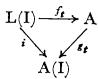
\includegraphics[keepaspectratio]{images/part001_16682a88.jpg}}

其中 \(i\) 是典范单射， \(f_{t}\) 是由 \(\pmb{t}\) 定义的李代数同态，而 \(g_{t}\) 是使得 \(g_{t}(i) = t_{i}\) （对 \(i\in I\) ）的幺代数同态。由于 \(g_{t}\circ i\) 与 \(f_{t}\) 在 I 上一致，该图表是交换的。由此得出，若 \(\mathrm{P}\in \mathrm{L}(\mathrm{I})\) ，则 § 2 no. 4 中定义的元素 \(\mathrm{P}((t_i)_{i\in I})\) 与《代数》第 III 章 § 2 no. 8 例 2 中定义的元素 \(\mathrm{P}((t_i)_{i\in I})\) 一致。

\subsection{\texorpdfstring{\(A^{+}(\mathrm{X})\) 到 \(\mathrm{L}(\mathrm{X})\) 上的投影}{A+ (X) 到 L(X) 上的投影}}

设 \(\pi\) 是 \(A^{+}(X)\) 到 \(L(X)\) 中的由下式定义的线性映射

\[
\pi (x _ {1} \dots x _ {n}) = (\mathrm{ad} (x _ {1}) \circ \dots \circ \mathrm{ad} (x _ {n - 1})) (x _ {n})\tag{3}
\]

其中 X 中的 \(n \geqslant 1, x_1, \ldots, x_n\) 。

命题 1. (a) 限制 \(\pi_0\) （即 \(\pi\) 在 \(\mathrm{L}(\mathbf{X})\) 上的限制）是 \(\mathrm{L}(\mathbf{X})\) 的一个导子。

\begin{enumerate}
\def\labelenumi{(\alph{enumi})}
\setcounter{enumi}{1}
\item
  对每个整数 \(n \geqslant 1\) 以及一切 \(u\) （属于 \(\mathbf{L}^n(\mathbf{X})\) ）， \(\pi(\mathbf{u}) = n.u.\)
\item
  设 E 是模 L(X) 的自同态代数， \(\theta\) 是 A(X) 到 E 中的一个同态，使得 \(\theta(x) = \operatorname{ad} x\) （对一切 \(x \in X\) ）。 \(\theta\) 在 L(X) 上的限制是 L(X) 到 E 中的一个李代数同态，它在 X 上与 L(X) 的伴随表示一致，从而
\end{enumerate}

\[
\theta (u). v = [ u, v ] \quad \text { for   } u, v \text {   in   } L (X).\tag{4}
\]

设 \(a\) 属于 \(\mathrm{A}(\mathrm{X})\) ， \(b\) 属于 \(\mathrm{A}^{+}(\mathrm{X})\) ；则

\[
\pi (a. b) = \theta (a). \pi (b).\tag{5}
\]

只需考虑 \(a = x_{1} \ldots x_{p}\) 、 \(b = x_{p+1} \ldots x_{p+q}\) （其中 \(p \geqslant 0\) ）、 \(q \geqslant 1\) 以及 \(x_{1}, \ldots, x_{p+q}\) （属于 \(\mathbf{X}\) ）的情形；但这时 (5) 由 (3) 立即得出，因为 \(\theta(x) = \operatorname{ad} x\) （对 \(x \in \mathbf{X}\) ）。

设 \(u\) 与 \(v\) 属于 \(\mathbf{L}(\mathbf{X})\) ；由 (4) 与 (5)，

\[
\begin{array}{r l} \pi_ {0} ([ u, v ]) & = \pi (u v - v u) = \theta (u). \pi (v) - \theta (v). \pi (u) \\ & = [ u, \pi (v) ] - [ v, \pi (u) ] = [ u, \pi_ {0} (v) ] + [ \pi_ {0} (u), v ], \end{array}
\]

因此 \(\pi_0\) 是 L(X) 的一个导子。

\begin{enumerate}
\def\labelenumi{(\alph{enumi})}
\setcounter{enumi}{1}
\tightlist
\item
  设 \(\pi_1\) 是模 \(\mathrm{L}(\mathbf{X})\) 的这样一个自同态：它在 \(\mathrm{L}^n (\mathbf{X})\) 上与用整数 \(n\geqslant 1\) 作乘法一致。公式 \([\mathrm{L}^n (\mathbf{X}),\mathrm{L}^m (\mathbf{X})]\subset \mathrm{L}^{n + m}(\mathrm{X})\) 表明 \(\pi_{1}\) 是一个导子 (《代数》， 第 III 章， § 10， no. 3， 例 6)。导子 \(\pi_1 - \pi_0\) （\(\mathrm{L}(\mathbf{X})\) 的）在 \(\mathbf{X}\) 上为零，并且由于 \(\mathbf{X}\) 生成 \(\mathrm{L}(\mathbf{X}),\pi_0 = \pi_1\) ，由此得 (b)。
\end{enumerate}

推论. 假设 K 是一个 Q-代数。设 P 是 \(A^{+}(X)\) 到其自身的线性映射，使得

\[
\mathrm{P} \left(x _ {1} \dots x _ {n}\right) = \frac {1}{n} (\operatorname{ad} x _ {1} \circ \dots \circ \operatorname{ad} x _ {n - 1}) (x _ {n})\tag{6}
\]

其中 \(n \geqslant 1\) 与 \(x_1, \ldots, x_n\) 都属于 \(\mathbf{X}\) 。那么 \(\mathbf{P}\) 是 \(\mathbf{A}^+(\mathbf{X})\) 到 \(\mathbf{L}(\mathbf{X})\) 上的一个投影。

\(\mathbf{P}\) 的像包含在 \(\mathrm{L}(\mathrm{X})\) 中。此外，对一切 \(n \geqslant 1\) 以及一切 \(u\) （属于 \(\mathrm{L}^n (\mathrm{X})\) ），有 \(\mathrm{P}(u) = \frac{1}{n}\pi (u)\) ，从而由命题 1 得 \(\mathrm{P}(u) = u\) 。由于

\[
\mathrm{L} (\mathrm{X}) = \sum_ {n \geqslant 1} \mathrm{L} ^ {n} (\mathrm{X}),
\]

我们看出 P 在 L(X) 上的限制是恒同映射。

注. 假设 K 是一个特征为零的域，并设 Q 是与 U(L(X)) 的典范分次相伴的、A(X) = U(L(X)) 到 L(X) 上的投影，参见 § 1 no. 5。对 \(\alpha \in \mathbf{N}^{(\mathbf{X})}\) ，有 Q(A \(^\alpha\) (X)) ⊂ L \(^\alpha\) (X)。因为只需验证 Q 的像与核都是 A(X) 的带有 N 型 \(^\alpha\) 分次的分次子模。这对像是显然的，因为它等于 L(X)。另一方面，设 n 是一个整数 \(\geqslant\) 1。A(X) 的由诸 \(y^n\) （其中 \(y \in L\) (X)）生成的向量子空间等于 A(X) 的由诸 \(\sum_{\sigma \in \mathcal{E}_n} y_{\sigma(1)} y_{\sigma(2)} \ldots y_{\sigma(n)}\) （其中 \(y_1, y_2, \ldots, y_n\) 是 L(X) 的齐次元素）生成的向量子空间；于是这个子空间是 A(X) 的一个分次子模。

（注意，若 \(\operatorname{Card}(\mathbf{X}) \geqslant 2\) ，则投影 \(\mathbf{P}\) 与 \(\mathbf{Q}\) 在 \(\mathbf{A}^{+}(\mathbf{X})\) 上并不一致。因为设 \(x, y\) 属于 \(\mathbf{X}\) 且 \(x \neq y\) ，并写

\[
z = x [ x, y ] + [ x, y ] x = x ^ {2} y - y x ^ {2}.
\]

则 \(\mathbf{Q}(z) = 0\) 且 \(\mathrm{P}(z) = \frac{1}{3}[x, [x,y]] \neq 0\) ，参见 § 2 no. 10 的例以及 no. 11 的定理 1。）

\subsection{L(X) 的齐次分量的维数}

设 X 是一个集合， \(\alpha\) 是 \(\mathbf{N}^{(X)}\) 的一个元素，d 是一个 >0 的整数。我们记 \(d|\alpha\) ，如果存在 \(\beta\in\mathbf{N}^{(X)}\) 使得 \(\alpha=d\beta\) 。这时唯一的元素 \(\beta\) 记作 \(\alpha/d\) 。

引理 1. 设 \(n\) 是一个整数 \(>0\) ， \(T_1, \ldots, T_n\) 是不定元， \(u_1, \ldots, u_n\) 是 \(\mathbf{Z}\) 的元素。设 \((c(\alpha))_{\alpha \in \mathbf{N}^n - \{0\}}\) 是 \(\mathbf{Z}\) 的元素的一个族，使得

\[
1 - \sum_ {i = 1} ^ {n} u _ {i} T _ {i} = \prod_ {\alpha \neq 0} (1 - T ^ {\alpha}) ^ {c (\alpha)}.\tag{7}
\]

对一切 \(\alpha \in \mathbf{N}^n - \{0\}\) ，

\[
c (\alpha) = \frac {1}{| \alpha |} \sum_ {d | \alpha} \mu (d) \frac {(| \alpha | / d) !}{(\alpha / d) !} u ^ {\alpha / d}\tag{8}
\]

其中 \(\mu\) 是 Möbius 函数（附录）。

在两边取对数后 (《代数》， 第 IV 章， § 6， no. 9)，公式 (7) 等价于：

\[
\log \left(1 - \sum_ {i = 1} ^ {n} u _ {i} T _ {i}\right) = \sum_ {\alpha \neq 0} c (\alpha) \log (1 - T ^ {\alpha}).\tag{9}
\]

而

\[
\begin{array}{r l} - \log \left(1 - \sum_ {i = 1} ^ {n} u _ {i} \mathrm{T} _ {i}\right) & = \sum_ {j \geqslant 1} \frac {1}{j} \left(\sum_ {i = 1} ^ {n} u _ {i} \mathrm{T} _ {i}\right) ^ {j} \\ & = \sum_ {j \geqslant 1} \frac {1}{j} \sum_ {| \beta | = j} \frac {| \beta | !}{\beta !} u ^ {\beta} \mathrm{T} ^ {\beta} \\ & = \sum_ {| \beta | > 0} \frac {1}{| \beta |} \frac {| \beta | !}{\beta !} u ^ {\beta} \mathrm{T} ^ {\beta}. \end{array}\tag{10}
\]

另一方面

\[
\begin{array}{r l} - \sum_ {\alpha \neq 0} c (\alpha) \log (1 - T ^ {\alpha}) & = \sum_ {| \alpha | > 0, k \geqslant 1} \frac {1}{k} c (\alpha) T ^ {k \alpha} \\ & = \sum_ {| \beta | > 0, k | \beta} \frac {1}{k} c \left(\frac {\beta}{k}\right) T ^ {\beta}. \end{array}\tag{11}
\]

因此 (7) 等价于

\[
\sum_ {k \mid \beta} \left| \frac {\beta}{k} \right| c \left(\frac {\beta}{k}\right) = \frac {| \beta | !}{\beta !} u ^ {\beta} \quad \text { for   all } \beta \in \mathbf {N} ^ {n} - \{0 \}.\tag{12}
\]

设 \(\Lambda\) 是由 \((\lambda_1, \lambda_2, \ldots, \lambda_n) \in \mathbf{N}^n - \{0\}\) 组成的集合，其中 \(\lambda_1, \lambda_2, \ldots, \lambda_n\) 的最大公因子等于 1。 \(\mathbf{N}^n - \{0\}\) 的每个元素都可以唯一地写成

形式 \(m\lambda\) ，其中 \(m\) 是一个整数 \(\geqslant 1\) 且 \(\lambda \in \Lambda\) 。条件 (12) 等价于

\[
\sum_ {k \mid m} \left| \frac {m \lambda}{k} \right| c \left(\frac {m \lambda}{k}\right) = \frac {(m | \lambda |) !}{(m \lambda) !} u ^ {m \lambda} \quad \text { for   all } \lambda \in \Lambda \text { and   all } m \geqslant 1.\tag{13}
\]

由 Möbius 反演公式（附录），条件 (13) 等价于

\[
\left| m \lambda \right| c (m \lambda) = \sum_ {d \mid m} \mu (d) \frac {\left| \frac {m \lambda}{d} \right| !}{\left(\frac {m \lambda}{d}\right) !} u ^ {\frac {m \lambda}{d}}\tag{14}
\]

其中一切 \(\lambda\in\Lambda\) 与一切 \(m\geqslant1\) 。

定理 2. 设 X 是一个有限集，并且 \(n = \operatorname{Card}(X)\) 。

\begin{enumerate}
\def\labelenumi{(\alph{enumi})}
\tightlist
\item
  对每个整数 \(r \geqslant 1\) ，K-模 \(\mathbf{L}^r(\mathbf{X})\) 都是自由的，其秩为
\end{enumerate}

\[
c (r) = \frac {1}{r} \sum_ {d | r} \mu (d) n ^ {r / d},\tag{15}
\]

其中 μ 是 Möbius 函数。

\begin{enumerate}
\def\labelenumi{(\alph{enumi})}
\setcounter{enumi}{1}
\tightlist
\item
  对一切 \(\alpha \in \mathbf{N}^{(\mathbf{X})} - \{0\}\) ，K-模 \(\mathbf{L}^{\alpha}(\mathbf{X})\) ( \(\S 2\) ， no. 6) 都是自由的，其秩为
\end{enumerate}

\[
c (\alpha) = \frac {1}{| \alpha |} \sum_ {d | \alpha} \mu (d) \frac {(| \alpha | / d) !}{(\alpha / d) !}.\tag{16}
\]

我们已经知道，模 \(L^{r}(\mathbf{X})\) （其中 \(r \in \mathbf{N}\) ）与 \(L^{\alpha}(\mathbf{X})\) （其中 \(\alpha \in \mathbf{N}^{\mathbf{X}}\) ）都是自由的 (§ 2， no. 11， 定理 1 的推论)。考察 A(X) 的多重分次 \((A^{\alpha}(X))_{\alpha \in \mathbf{N}^{\mathbf{X}}}\) ，它由典范同态 \(\phi\) （从 Mo(X) 到 \(\mathbf{N}^{\mathbf{X}}\) 中）所定义 (《代数》， 第 III 章， § 3， no. 1， 例 3)；于是由 no. 1 的注 3 有 \(A^{\alpha}(\mathbf{X}) \cap L(\mathbf{X}) = L^{\alpha}(\mathbf{X})\) 。对 \(\alpha \in \mathbf{N}^{\mathbf{X}}\) ，K-模 \(A^{\alpha}(\mathbf{X})\) 以这样的字的集合为基：X 的每个字母 \(x\) 在其中出现 \(\alpha(x)\) 次。设 \(d(\alpha)\) 是这些字的个数，即 \(A^{\alpha}(\mathbf{X})\) 的秩；我们将以两种不同的方式计算形式幂级数

它由

\[
\mathbf {P} ((\mathrm{T} _ {x}) _ {x \in \mathbf {X}}) \in \mathbf {Z} [ [ (\mathrm{T} _ {x}) _ {x \in \mathbf {X}} ] ]\tag{17}
\]

\[
\mathrm{P} (\mathrm{T}) = \sum_ {\alpha \in \mathbf {N} ^ {\mathbf {X}}} d (\alpha) \mathrm{T} ^ {\alpha}.
\]

\begin{enumerate}
\def\labelenumi{(\arabic{enumi})}
\tightlist
\item
  我们有
\end{enumerate}

\[
\mathrm{P} (\mathrm{T}) = \sum_ {m \in \mathrm{Mo} (\mathrm{X})} \mathrm{T} ^ {\phi (m)} = \sum_ {r = 0} ^ {\infty} \sum_ {x _ {1}, \dots , x _ {r}} \mathrm{T} _ {x _ {1}} \dots \mathrm{T} _ {x _ {r}} = \sum_ {r = 0} ^ {\infty} \left(\sum_ {x \in \mathrm{X}} \mathrm{T} _ {x}\right) ^ {r}
\]

从而

\[
\mathrm{P} (\mathrm{T}) = \left(1 - \sum_ {x \in \mathbf {X}} \mathrm{T} _ {x}\right) ^ {- 1}.\tag{18}
\]

\begin{enumerate}
\def\labelenumi{(\arabic{enumi})}
\setcounter{enumi}{1}
\tightlist
\item
  对一切 \(\alpha \in \mathbf{N}^{\mathbf{X}} - \{0\}\) ，设 \((e_{\alpha,j})_{1 \leqslant j \leqslant c(\alpha)}\) 是 \(\mathrm{L}^{\alpha}(\mathbf{X})\) 的一个基，并给集合 I 一个全序，I 由有序对 \((\alpha, j)\) （满足 \(\alpha \in \mathbf{N}^{\mathbf{X}} - \{0\}\) 且 \(1 \leqslant j \leqslant c(\alpha)\) ）组成。由 no. 1 的定理 1 与 Poincaré-Birkhoff-Witt 定理 (第 I 章， § 2， no. 7， 定理 1 的推论 3)，诸元素
\end{enumerate}

\[
y _ {m} = \prod_ {(\alpha , j) \in \mathbb {I}} (e _ {\alpha , j}) ^ {m (\alpha , j)},
\]

（其中指标 \(\pmb{m}\) 取遍 \(\mathbf{N}^{(I)}\) ）构成 \(A(\mathbf{X})\) 的一个基。每个 \(y_{m}\) 都有一个多重次数 \(\sum_{(\alpha, j) \in I} \pmb{m}(\alpha, j)\alpha\) 。用 \(u(\pmb{m})\) 表示这个多重次数。由此得出

\[
\begin{array}{l} \mathrm{P(T)} = \sum_ {m \in \mathrm{N} ^ {(I)}} \mathrm{T} ^ {u (m)} = \sum_ {m \in \mathrm{N} ^ {(I)}} \prod_ {(\alpha , j) \in I} \mathrm{T} ^ {m (\alpha , j) \alpha} \\ = \prod_ {(\alpha , j) \in I} \sum_ {r = 0} ^ {\infty} \mathrm{T} ^ {r \alpha} = \prod_ {(\alpha , j) \in I} (1 - \mathrm{T} ^ {\alpha}) ^ {- 1}, \end{array}
\]

从而最后

\[
\mathrm{P} (\mathrm{T}) = \prod_ {\alpha \in \mathbf {N} ^ {\mathbf {X}} - \{0 \}} (1 - \mathrm{T} ^ {\alpha}) ^ {- c (\alpha)}.\tag{19}
\]

比较 (18) 与 (19)，我们得到

\[
1 - \sum_ {x \in \mathbf {X}} T _ {x} = \prod_ {\alpha \in \mathbf {N} ^ {\mathbf {X}} - \{0\}} (1 - T ^ {\alpha}) ^ {c (\alpha)}.\tag{20}
\]

于是引理 1 给出 (b)。

若现在在公式 (20) 中把同一个不定元 U 代入诸 \(T_{x}\) （对 \(x \in X\) ），则得到

\[
1 - n \mathrm{U} = \prod_ {\alpha \in \mathbf {N} ^ {\mathrm{X}} - \{0\}} (1 - \mathrm{U} ^ {| \alpha |}) ^ {c (\alpha)} = \prod_ {r > 0} (1 - \mathrm{U} ^ {r}) ^ {c (r)}.
\]

再次应用引理 1，我们推出 (a)。

例. 我们有

\[
\begin{array}{l l} c (1) = n, & c (2) = \frac {1}{2} (n ^ {2} - n), \qquad c (3) = \frac {1}{3} (n ^ {3} - n), \\ c (4) = \frac {1}{4} (n ^ {4} - n ^ {2}), & c (5) = \frac {1}{5} (n ^ {5} - n), \qquad c (6) = \frac {1}{6} (n ^ {6} - n ^ {3} - n ^ {2} + n). \end{array}
\]

注. 设 X 是一个集合并设 \(\alpha \in \mathbf{N}^{(X)}\) ；自由 K-模 \(\mathbf{L}^{\alpha}(X)\) 的秩也由公式 (16) 给出。这由定理 2 (b) 以及 § 2 no. 6 的命题 4 立即得出。

\section{中心滤过}

\subsection{实滤过}

定义 1. 设 G 是一个群。G 上的实滤过是指 G 的子群的一个族 \((\mathrm{G}_{\alpha})_{\alpha \in \mathbf{R}}\) ，使得

\[
\mathrm{G} _ {\alpha} = \bigcap_ {\beta <   \alpha} \mathrm{G} _ {\beta} \text {   for   all   } \alpha \in \mathbf {R}.\tag{1}
\]

公式 (1) 蕴涵 \(G_{\alpha} \subset G_{\beta}\) （对 \(\beta < \alpha\) ），因而族 \((\mathrm{G}_{\alpha})\) 是递减的。滤过 \((\mathrm{G}_{\alpha})\) 称为分离的，如果 \(\bigcap_{\alpha} G_{\alpha}\) 化为单位元素；称为穷竭的，如果 \(G = \bigcup_{\alpha} G_{\alpha}\) 。

注. 设 \((\mathrm{G}_n)_{n\in \mathbf{Z}}\) 是 G 的子群的一个递减序列。它是《交换代数》第 III 章 § 2 no. 1 定义 1 意义下的递减滤过。对每个整数 \(n\) 以及每个 \(\alpha\) （取自区间 \(]n - 1,n]\) ，即 \(\mathbf{R}\) 中的一个区间），我们记 \(\mathrm{H}_{\alpha} = \mathrm{G}_{n}\) ，特别地 \(\mathrm{H}_n = \mathrm{G}_n\) 。立即可见我们这样就得到 G 上的一个实滤过 \((\mathrm{H}_{\alpha})_{\alpha \in \mathbf{R}}\) ；这样的滤过将称为整滤过。因此《交换代数》第 III 章 § 2 意义下的递减滤过可以与整滤过等同。

设 A 是一个代数；A 的加法群上的实滤过 \((\mathrm{A}_{\alpha})\) 称为与该代数结构相容，如果 \(\mathrm{A}_{\alpha}.\mathrm{A}_{\beta}\subset \mathrm{A}_{\alpha +\beta}\) （对 R 中的 \(\alpha ,\beta\) ），且 \(\mathrm{K.A}_{\alpha}\subset \mathrm{A}_{\alpha}\) （对 \(\alpha \in \mathbf{R}\) ）。若滤过是穷竭的，则 \((\mathrm{A}_{\alpha})\) 是 A 上与该代数结构相容的拓扑之下 0 的一个邻域基本系。设 B 是一个幺代数；B 的加法群上的实滤过 \((\mathrm{B}_{\alpha})\) 称为与该幺代数结构相容，如果它与该代数结构相容并且 \(1\in \mathrm{B}_0\) 。

\subsection{阶函数}

设 \(G\) 是一个以 \(e\) 为单位元素的群。设 \((\mathbf{G}_{\alpha})\) 是 \(G\) 上的一个实滤过。对一切 \(x\) （属于 \(G\) ），用 \(I_x\) 表示实数 \(\alpha\) 组成的集合，其中实数满足 \(x \in G_{\alpha}\) 。若 \(\alpha \in I_x\) 且 \(\beta < \alpha\) ，则 \(\beta \in I_x\) ，因而 \(I_x\) 是一个区间 (《一般拓扑学》， 第 IV 章， § 2， no. 4， 命题 1)。利用关系式 (1)，我们看出 \(I_x\) 当其上确界有限时含有该上确界。因此 \(I_x\) 具有形式 \(] - \infty\) 、 \(v(x)] \cap R\) ，其中 \(v(x) \in \overline{\mathbf{R}}\) ；我们有 \(v(x) = \sup(\alpha \mid x \in G_{\alpha})\) 。

映射 \(v\) （从 \(G\) 到 \(\overline{\mathbf{R}}\) 中）称为与实滤过 \((G_{\alpha})\) 相伴的阶函数，而 \(v(x)\) 称为 \(x\) 的阶。这个映射具有下列性质：

\begin{enumerate}
\def\labelenumi{(\alph{enumi})}
\item
  对 \(x \in \mathbf{G}\) 与 \(\alpha \in \mathbf{R}\) ，关系式 \(x \in \mathbf{G}_{\alpha}\) 与 \(v(x) \geqslant \alpha\) 等价。
\item
  对 G 中的 x、y，
\end{enumerate}

\begin{enumerate}
\def\labelenumi{(\arabic{enumi})}
\setcounter{enumi}{1}
\tightlist
\item
\end{enumerate}

\[
v (x ^ {- 1}) = v (x), \quad v (e) = + \infty .\tag{2}
\]

\[
v (x y) \geqslant \inf (v (x), v (y)).\tag{3}
\]

此外，当 \(v(x) > v(y)\) 时 (3) 中取等号。

\begin{enumerate}
\def\labelenumi{(\alph{enumi})}
\setcounter{enumi}{2}
\tightlist
\item
  对一切 \(\alpha \in \mathbf{R}\) ，用 \(\mathrm{G}_{\alpha}^{+}\) 表示 \(x \in \mathrm{G}\) 组成的集合，其中 \(v(x) > \alpha\) 。那么 \(\mathrm{G}_{\alpha}^{+} = \bigcup_{\beta > \alpha} \mathrm{G}_{\beta}\) ，特别地 \(\mathrm{G}_{\alpha}^{+}\) 是 \(\mathrm{G}\) 的一个子群。
\end{enumerate}

反之，设 \(v\) 是 \(G\) 到 \(\overline{\mathbf{R}}\) 中的满足关系式 (2) 与 (3) 的映射。对一切 \(\alpha \in \mathbf{R}\) ，令 \(G_{\alpha}\) 为 \(x \in G\) 组成的集合，其中 \(v(x) \geqslant \alpha\) 。那么 \((G_{\alpha})_{\alpha \in \mathbf{R}}\) 是 \(G\) 的一个实滤过，而 \(v\) 是与这个滤过相伴的阶函数。

滤过 \((\mathbf{G}_{\alpha})\) 为整滤过，当且仅当 \(v\) 把 \(\mathbf{G}\) 映到 \(\mathbf{Z} \cup \{+\infty, -\infty\}\) 中。它为穷竭的（相应地，分离的），当且仅当 \(v^{-1}(-\infty) = \varnothing\) （相应地， \(v^{-1}(+\infty) = \{e\}\) ）。

设 A 是一个 K-代数（相应地，幺 K-代数）。由上所述，关系式

\[
" x \in \mathrm{A} _ {\alpha} \Leftrightarrow v (x) \geqslant \alpha \quad \text { for } x \in \mathrm{A} \text { and } \alpha \in \mathbf {R}"
\]

定义了 A 上与代数（相应地，幺代数）结构相容的穷竭实滤过 \((\mathbf{A}_{\alpha})_{\alpha\in\mathbf{R}}\) 的集合到映射 \(v: A \to \overline{\mathbf{R}}\) 组成的集合上的一个双射，这些映射不取值 \(-\infty\) 且满足下列公理 (4) 至 (7)（相应地， (4) 至 (8)）：

\begin{enumerate}
\def\labelenumi{(\arabic{enumi})}
\setcounter{enumi}{3}
\tightlist
\item
\end{enumerate}

\[
v (x + y) \geqslant \inf (v (x), v (y)) \quad (x, y \text {   in   A })\tag{5}
\]

\[
v (- x) = v (x) \quad (x \in \mathrm{A})\tag{6}
\]

\[
v (\lambda x) \geqslant v (x) \quad (\lambda \in \mathrm{K}, x \in \mathrm{A})\tag{7}
\]

\[
v (x y) \geqslant v (x) + v (y) \quad (x, y \text {   in   A })\tag{8}
\]

\[
v (1) \geqslant 0.
\]

注. 若 \(v(x)\) 不恒等于 \(+\infty\) ，则条件 (7) 与 (8) 蕴涵 \(v(1) = 0\) 。

\subsection{与滤过代数相伴的分次代数}

设 G 是一个带实滤过 \((G_{\alpha})_{\alpha \in \mathbb{R}}\) 的交换群。如同前面我们记

\[
\mathrm{G} _ {\alpha} ^ {+} = \bigcup_ {\beta > \alpha} \mathrm{G} _ {\beta};\tag{9}
\]

显然 \(\mathrm{G}_{\alpha}^{+}\) 是 \(\mathrm{G}_{\alpha}\) 的一个子群。我们记 \(\mathrm{gr}_{\alpha}(\mathrm{G}) = \mathrm{G}_{\alpha} / \mathrm{G}_{\alpha}^{+}\) ，并且

\[
\operatorname{gr} (\mathrm{G}) = \bigoplus_ {\alpha \in \mathbf {R}} \operatorname{gr} _ {\alpha} (\mathrm{G}).
\]

与滤过群 G 相伴的分次群是群 \(\operatorname{gr}(G)\) ，带其自然的 R 型分次。

注. 当滤过 \((\mathrm{G}_{\alpha})\) 是整滤过时， \(\mathrm{gr}_{\alpha}(\mathrm{G}) = \{0\}\) （对非整的 \(\alpha\) ），而 \(\mathrm{gr}_n(\mathrm{G}) = \mathrm{G}_n / \mathrm{G}_{n - 1}\) （对每个整数 \(n\) ）。因此相伴分次群的定义与《交换代数》第 III 章 § 2 no. 3 中的定义本质上是一致的。

设 \(\mathbf{A}\) 是一个代数（相应地，幺代数）， \((\mathbf{A}_{\alpha})_{\alpha \in \mathbb{R}}\) 是一个与代数（相应地，幺代数）结构相容的实滤过 (no. 1)。那么

\[
\mathrm{A} _ {\alpha}. \mathrm{A} _ {\beta} \subset \mathrm{A} _ {\alpha + \beta}, \quad \mathrm{A} _ {\alpha} ^ {+}. \mathrm{A} _ {\beta} + \mathrm{A} _ {\alpha}. \mathrm{A} _ {\beta} ^ {+} \subset \mathrm{A} _ {\alpha + \beta} ^ {+},
\]

，并且由 A 上乘法的限制所给出的 \(A_{\alpha} \times A_{\beta}\) 到 \(A_{\alpha+\beta}\) 中的双线性映射在取商后定义了一个双线性映射

\[
\operatorname{gr} _ {\alpha} (\mathrm{A}) \times \operatorname{gr} _ {\beta} (\mathrm{A}) \rightarrow \operatorname{gr} _ {\alpha + \beta} (\mathrm{A}).
\]

我们得到 \(\mathrm{gr}(\mathbf{A}) \times \mathrm{gr}(\mathbf{A})\) 到 \(\mathrm{gr}(\mathbf{A})\) 中的一个双线性映射，它使后者成为一个 R 型分次代数（相应地，幺分次代数）。若 A 是一个结合代数（相应地，交换代数，相应地，李代数），则 \(\mathrm{gr}(\mathbf{A})\) 亦然。

\subsection{群上的中心滤过}

定义 2. 设 G 是一个群。G 上的实滤过 \((\mathrm{G}_{\alpha})\) 称为中心的，如果 \(\mathrm{G} = \bigcup_{\alpha >0}\mathrm{G}_{\alpha}\) ，并且换位子 \((x,y) = x^{-1}y^{-1}xy\) ——它由一个元素 \(x\) （属于 \(\mathrm{G}_{\alpha}\) ）与一个元素 \(y\) （属于 \(\mathrm{G}_{\beta}\) ）构成——属于 \(\mathrm{G}_{\alpha +\beta}\) 。

用阶函数 v 来说，上述定义转换为关系式

\[
v (x) > 0, \quad v ((x, y)) \geqslant v (x) + v (y) \quad \text { for   all } x, y \text { in } G.\tag{10}
\]

我们推出 \(v((x,y)) > v(x)\) （若 \(v(x) \neq +\infty\) ）；若记 \(x^y = y^{-1}xy\) （参见《代数》， 第 I 章， § 6， no. 2），则 \(x^y = x.(x,y)\) ，从而

\[
v (x ^ {y}) = v (x).\tag{11}
\]

这个关系式表达了如下事实：G 的诸子群 \(G_{\alpha}\) 中的每一个都是正规的。诸 \(G_{\alpha}\) 构成与 G 上群结构相容的一个拓扑 (《一般拓扑学》， 第 III 章， § 1， no. 2， 例) 之下 e 的一个邻域基本系，该拓扑称为由滤过 ( \(G_{\alpha}\) ) 所定义。

在本 no. 的其余部分，G 表示一个带中心滤过 \((G_{\alpha})\) 的群。对一切 \(\alpha \in R\) ，我们用下式定义 G 的子群 \(G_{\alpha}^{+}\) ：

\[
\mathrm{G} _ {\alpha} ^ {+} = \bigcup_ {\beta > \alpha} \mathrm{G} _ {\beta}.\tag{12}
\]

特别地， \(G_{\alpha}^{+} = G_{\alpha} = G\) （对 \(\alpha \leqslant 0\) ）。回顾若 A 与 B 是 G 的两个子群，则 (A, B) 表示由换位子 \((a, b)\) （满足 \(a \in A\) 且 \(b \in B\) ）生成的 G 的子群。用这个记号，我们有公式

\begin{enumerate}
\def\labelenumi{(\arabic{enumi})}
\setcounter{enumi}{12}
\tightlist
\item
\end{enumerate}

\[
\left(\mathrm{G} _ {\alpha}, \mathrm{G} _ {\beta}\right) \subset \mathrm{G} _ {\alpha + \beta}\tag{13}
\]

\[
\left(\mathrm{G} _ {\alpha} ^ {+}, \mathrm{G} _ {\beta}\right) \subset \mathrm{G} _ {\alpha + \beta} ^ {+}\tag{13'}
\]

\[
(G, G _ {\alpha}) \subset G _ {\alpha} ^ {+}.\tag{14}
\]

由 (14)， \(\mathrm{G}_{\alpha}^{+}\) 是 \(\mathrm{G}_{\alpha}\) 的一个正规子群（对一切 \(\alpha \in \mathbf{R}\) ），并且商群 \(\mathrm{gr}_{\alpha}(\mathrm{G}) = \mathrm{G}_{\alpha} / \mathrm{G}_{\alpha}^{+}\) 是交换的。我们记 \(\mathrm{gr}(\mathrm{G}) = \bigoplus_{\alpha \in \mathbb{R}}\mathrm{gr}_{\alpha}(\mathrm{G})\) ，并给这个群赋予 \(\mathbf{R}\) 型分次，其中 \(\mathrm{gr}_{\alpha}(\mathrm{G})\) 由 \(\alpha\) 次的元素组成。于是 \(\mathrm{gr}_{\alpha}(\mathrm{G}) = \{0\}\) （对 \(\alpha \leqslant 0\) ）。

命题 1. (i) 设 \(\alpha, \beta\) 属于 \(\mathbf{R}\) 。存在一个双加性映射

\[
\phi_ {\alpha \beta}: \operatorname{gr} _ {\alpha} (\mathrm{G}) \times \operatorname{gr} _ {\beta} (\mathrm{G}) \rightarrow \operatorname{gr} _ {\alpha + \beta} (\mathrm{G})
\]

它把 \((x\mathrm{G}_{\alpha}^{+},y\mathrm{G}_{\beta}^{+})\) 映到 \((x,y)\mathrm{G}_{\alpha +\beta}^{+}\) 上

\begin{enumerate}
\def\labelenumi{(\roman{enumi})}
\setcounter{enumi}{1}
\item
  设 \(\phi\) 是 \(\operatorname{gr}(\mathbf{G}) \times \operatorname{gr}(\mathbf{G})\) 到 \(\operatorname{gr}(\mathbf{G})\) 中的一个双加性映射，它在 \(\operatorname{gr}_{\alpha}(\mathbf{G}) \times \operatorname{gr}_{\beta}(\mathbf{G})\) 上的限制是 \(\phi_{\alpha \beta}\) （对每个有序对 \((\alpha, \beta)\) ）。映射 \(\phi\) 给 \(\operatorname{gr}(\mathbf{G})\) 一个李 Z-代数结构。
\item
  回顾恒等式
\end{enumerate}

\[
(x x ^ {\prime}, y) = (x, y) ^ {x ^ {\prime}} \left(x ^ {\prime}, y\right)\tag{15}
\]

其中 \(x, x', y\) 属于 \(\mathbf{G}\) (《代数》， 第 I 章， § 6， no. 2， 公式 (4 bis))。

对 \(x \in G_{\alpha}\) 与 \(y \in G_{\beta}\) ，模 \(G_{\alpha + \beta}^{+}\) 的类（元素 \((x, y)\) 取自 \(G_{\alpha + \beta}\) ）将记作 \(f(x, y)\) 。对 \(a\) （属于 \(G_{\alpha + \beta}\) ）与 \(x'\) （属于 \(G, a^{-1}.a^{x'} = (a, x') \in G_{\alpha + \beta}^{+}\) ）；特别地， \(f(x, y)\) 等于模 \(G_{\alpha + \beta}^{+}\) 的类（元素 \((x, y)^{x'}\) 的类）。因此公式 (15) 蕴涵

\[
f (x x ^ {\prime}, y) = f (x, y) f (x ^ {\prime}, y).\tag{16}
\]

而 \((y, x) = (x, y)^{-1}\) ，从而

\[
f (y, x) = f (x, y) ^ {- 1}.\tag{17}
\]

由 (16) 与 (17) 我们推出

\[
f (x, y y ^ {\prime}) = f (x, y) f (x, y ^ {\prime}).\tag{18}
\]

我们必须证明映射 \(f\colon \mathrm{G}_{\alpha}\times \mathrm{G}_{\beta}\to \mathrm{gr}_{\alpha +\beta}(\mathrm{G})\) 在取商后定义一个映射 \(\phi_{\alpha \beta}\colon \mathrm{gr}_{\alpha}(\mathrm{G})\times \mathrm{gr}_{\beta}(\mathrm{G})\to \mathrm{gr}_{\alpha +\beta}(\mathrm{G})\) 。由 (16) 与 (18)，只需证明 \(f(x,y) = 0\) （当 \(x\in \mathrm{G}_{\alpha}^{+}\) 或 \(y\in \mathrm{G}_{\beta}^{+}\) 时），而这由 (13') 得出。

\begin{enumerate}
\def\labelenumi{(\roman{enumi})}
\setcounter{enumi}{1}
\tightlist
\item
  由于 \((x, x) = e\) ，由 (17) 推出 \(\phi\) 是一个交错的双 \(\mathbf{Z}\) -线性映射。因此剩下要证明的是，对 \(u \in \mathrm{gr}_{\alpha}(\mathrm{G})\) 、 \(v \in \mathrm{gr}_{\beta}(\mathrm{G})\) 与 \(w \in \mathrm{gr}_{\gamma}(\mathrm{G})\) ，
\end{enumerate}

\[
\phi (u, \phi (v, w)) + \phi (v, \phi (w, u)) + \phi (w, \phi (u, v)) = 0.\tag{19}
\]

设 \(x \in G_{\alpha}, y \in G_{\beta}\) 与 \(z \in G_{\gamma}\) 是分别表示 \(u, v\) 与 \(w\) 的元素。我们知道 \(x^{y}\) 与 \(x\) 是 \(G_{\alpha}\) 的两个模 \(G_{\alpha}^{+}\) 同余的元素，因而 \(x^{y}\) 是 \(u\) 在 \(G_{\alpha}\) 中的一个代表；由于 \((y, z)\) 是 \(\phi(v, w)\) 在 \(G_{\beta + \gamma}\) 中的一个代表，我们看出 \((x^{y}, (y, z))\) 是 \(\phi(u, \phi(v, w))\) 在 \(G_{\alpha + \beta + \gamma}\) 中的一个代表。通过轮换，我们看出 \((y^{z}, (z, x))\) 与 \((z^{x}, (x, y))\) 分别表示 \(\phi(v, \phi(w, u))\) 与 \(\phi(w, \phi(u, v))\) （在 \(G_{\alpha + \beta + \gamma}\) 中）。于是关系式 (19) 是下列恒等式 (《代数》， 第 I 章， § 6， no. 2， 公式 (15)) 的推论：

\[
\left(x ^ {y}, (y, z)\right). \left(y ^ {z}, (z, x)\right). \left(z ^ {x}, (x, y)\right) = e.\tag{20}
\]

在命题 1 中定义的李代数 \(\mathrm{gr}(\mathbf{G})\) （环 \(\mathbf{Z}\) 上的）称为与滤过群 \(\mathbf{G}\) 相伴的分次李代数。

\subsection{中心滤过的一个例子}

设 \(\mathbf{A}\) 是一个带幺代数滤过 \((\mathbf{A}_{\alpha})\) 的幺结合代数，使得 \(\mathbf{A}_{0} = \mathbf{A}\) ；那么 \(\mathbf{A}_{\alpha}\) 是 \(\mathbf{A}\) 的一个双边理想（对一切 \(\alpha \in \mathbf{R}\) ）。用 \(\mathbf{A}^*\) 表示 \(\mathbf{A}\) 的可逆元素组成的乘法群。对一切 \(\alpha > 0\) ，用 \(\Gamma_{\alpha}\) 表示 \(x \in \mathbf{A}^*\) 组成的集合，其中 \(x - 1 \in \mathbf{A}_{\alpha}\) ；我们记 \(\Gamma = \bigcup_{\alpha > 0} \Gamma_{\alpha}\) 与 \(\Gamma_{\beta} = \Gamma\) （对 \(\beta \leqslant 0\) ）。

命题 2. 集合 \(\Gamma\) 是 \(\mathbf{A}^*\) 的一个子群，并且 \((\Gamma_{\alpha})\) 是 \(\Gamma\) 上的一个中心滤过。

按构造有 \(\Gamma = \bigcup_{\alpha > 0} \Gamma_{\alpha}\) ，而关系式 \(\Gamma_{\alpha} = \bigcap_{\beta < \alpha} \Gamma_{\beta}\) 由 \(A_{\alpha} = \bigcap_{\beta < \alpha} A_{\beta}\) 得出。

我们证明 \(\Gamma_{\alpha}\) 是 \(\mathbf{A}^*\) 的一个子群。而 \(1 \in \Gamma_{\alpha}\) ；设 \(x, y\) 属于 \(\Gamma_{\alpha}\) ，从而 \(x - 1 \in \mathbf{A}_{\alpha}, y - 1 \in \mathbf{A}_{\alpha}\) 。由于 \(\mathbf{A}_{\alpha}\) 是 \(\mathbf{A}\) 的一个双边理想，公式

\begin{enumerate}
\def\labelenumi{(\arabic{enumi})}
\setcounter{enumi}{20}
\tightlist
\item
\end{enumerate}

\[
x y - 1 = (x - 1) (y - 1) + (x - 1) + (y - 1),\tag{21}
\]

\[
x ^ {- 1} - 1 = - x ^ {- 1} (x - 1),\tag{22}
\]

蕴涵 \(xy - 1 \in A_{\alpha}\) 与 \(x^{-1} - 1 \in A_{\alpha}\) ，从而 \(xy \in \Gamma_{\alpha}\) 且 \(x^{-1} \in \Gamma_{\alpha}\) 。

由于 \(\Gamma = \bigcup_{\alpha > 0} \Gamma_{\alpha}\) ，它是 \(A^{*}\) 的一个子群。

最后设 \(\alpha > 0, \beta > 0, x \in \Gamma_{\alpha}\) 与 \(y \in \Gamma_{\beta}\) 。设 \(x - 1 = \xi\) 与 \(y - 1 = \eta\) 。那么

\[
(x, y) - 1 = x ^ {- 1} y ^ {- 1} (\xi \eta - \eta \xi);\tag{23}
\]

由假设， \(\xi \in \mathbf{A}_{\alpha}\) 且 \(\eta \in \mathbf{A}_{\beta}\) ，从而 \(\xi \eta - \eta \xi \in \mathbf{A}_{\alpha + \beta}\) 。由于 \(\mathbf{A}_{\alpha + \beta}\) 是 \(\mathbf{A}, (x, y) - 1 \in \mathbf{A}_{\alpha + \beta}\) 的一个双边理想，由此得 \((x, y) \in \Gamma_{\alpha + \beta}\) 。

注. 设 \(\alpha \geqslant 0, \beta \geqslant 0\) 与 \(x \in \Gamma_{\alpha}, y \in \Gamma_{\beta}\) 。由公式 (21)、 (22) 与 (23)，

\begin{enumerate}
\def\labelenumi{(\arabic{enumi})}
\setcounter{enumi}{23}
\tightlist
\item
\end{enumerate}

\[
x ^ {- 1} - 1 \equiv - (x - 1) \quad \text { mod. } A _ {2 \alpha}\tag{24}
\]

\[
x y - 1 \equiv (x - 1) + (y - 1) \quad \text { mod. } A _ {\alpha + \beta}\tag{25}
\]

\[
(x, y) - 1 \equiv [ (x - 1), (y - 1) ] \mod A _ {\alpha + \beta + \inf (\alpha , \beta)}.\tag{26}
\]

例如我们证明 (26)。若 \(x - 1 = \xi\) 且 \(y - 1 = \eta\) ，则 (23) 给出：

\[
(x, y) - 1 - [ \xi , \eta ] = ((x ^ {- 1} - 1) + (y ^ {- 1} - 1) + (x ^ {- 1} - 1) (y ^ {- 1} - 1)) [ \xi , \eta ].
\]

而 \([\xi, \eta] \in \mathrm{A}_{\alpha + \beta}, (x^{-1} - 1) \in \mathrm{A}_{\alpha}, (y^{-1} - 1) \in \mathrm{A}_{\beta}\) ，由此得到 (26)。

设 \(G\) 是一个群， \(\rho: G \to \Gamma\) 是一个同态。对一切实数 \(\alpha\) ，我们记 \(G_{\alpha} = \rho^{-1}(\Gamma_{\alpha})\) 。由于 \((\Gamma_{\alpha})\) 是 \(\Gamma\) 上的一个中心滤过，立即可见 \((G_{\alpha})\) 是 \(G\) 上的一个中心滤过。

命题 3. (i) 对一切 \(\alpha \in \mathbf{R}\) ，存在唯一的群同态 \(g_{\alpha} \colon \mathrm{gr}_{\alpha}(\mathrm{G}) \to \mathrm{gr}_{\alpha}(\mathrm{A})\) ，它把模 \(\mathrm{G}_{\alpha}^{+}\) 类（元素 \(a \in \mathrm{G}_{\alpha}\) 的类）映到模 \(\mathrm{A}_{\alpha}^{+}\) 类（\(\rho(a) - 1\) 的类）。

\begin{enumerate}
\def\labelenumi{(\roman{enumi})}
\setcounter{enumi}{1}
\item
  设 \(g\) 是 \(\mathrm{gr}(\mathrm{G})\) 到 \(\mathrm{gr}(\mathrm{A})\) 中的群同态，它在 \(\mathrm{gr}_{\alpha}(\mathrm{G})\) 上的限制是 \(g_{\alpha}\) （对一切 \(\alpha\) ）。映射 \(g\) 是李 Z-代数的一个单同态。 (i) 设 \(\alpha > 0\) 。由假设，结论对一切 \(a\) （属于 \(\mathrm{G}_{\alpha}, \rho(a) - 1 \in \mathrm{A}_{\alpha}\) ）成立；用 \(p_{\alpha}(a)\) 表示 \(\rho(a) - 1\) 模 \(\mathrm{A}_{\alpha}^{+}\) 的类。由于 \(\mathrm{A}_{\alpha} \subset \mathrm{A}_{\alpha}^{+}\) ，关系式 (25) 蕴涵 \(p_{\alpha}(ab) = p_{\alpha}(a) + p_{\alpha}(b)\) 。于是 \(a \in \mathrm{G}_{\alpha}^{+}\) 当且仅当 \(\rho(a) - 1 \in \mathrm{A}_{\alpha}^{+}\) ；因此 \(\mathrm{G}_{\alpha}^{+}\) 是同态 \(p_{\alpha}\) （从 \(\mathrm{G}_{\alpha}\) 到 \(\mathrm{gr}_{\alpha}(\mathrm{A})\) 中）的核。取商后， \(p_{\alpha}\) 便定义了一个单同态 \(g_{\alpha}\) （从 \(\mathrm{gr}_{\alpha}(\mathrm{G})\) 到 \(\mathrm{gr}_{\alpha}(\mathrm{A})\) 中）。对 \(\alpha \leqslant 0\) ，有 \(\mathrm{gr}_{\alpha}(\mathrm{G}) = \{0\}\) ，唯一的选择是 \(g_{\alpha} = 0\) 。
\item
  由于 \(g_{\alpha}\) 对一切实数 \(\alpha\) 都是单射， \(g\) 是单射。我们证明 \(g\) 是一个李代数同态。由于 \(\mathrm{gr}_{\alpha}(\mathrm{G}) = \{0\}\) （对 \(\alpha \leqslant 0\) ），只需建立公式
\end{enumerate}

\[
p _ {\alpha + \beta} ((a, b)) = [ p _ {\alpha} (a), p _ {\beta} (b) ]\tag{27}
\]

其中 \(\alpha > 0\) 、 \(\beta > 0\) 、 \(a \in G_{\alpha}\) 与 \(b \in G_{\beta}\) ，它由 (26) 得出。

\subsection{整中心滤过}

回顾 (no. 1， 注) 群 G 上的滤过 \((\mathrm{G}_{\alpha})\) 称为整的，如果 \(\mathrm{G}_{\alpha} = \mathrm{G}_{n}\) （对每个整数 \(n\) 以及一切 \(\alpha \in ]n - 1,n]\) ）。给定群 G 上的一个整中心滤过等价于给定 G 的子群的一个序列 \((\mathrm{G}_n)_{n\geqslant 1}\) ，它满足条件

\begin{enumerate}
\def\labelenumi{(\roman{enumi})}
\tightlist
\item
\end{enumerate}

\[
\mathrm{G} _ {1} = \mathrm{G}\tag{i}
\]

\[
\mathrm{G} _ {n} \supset \mathrm{G} _ {n + 1} \quad \text { for   all } n \geqslant 1\tag{ii}
\]

\[
\left(\mathrm{G} _ {m}, \mathrm{G} _ {n}\right) \subset \mathrm{G} _ {m + n} \quad \text { for } m \geqslant 1 \text { and } n \geqslant 1.\tag{iii}
\]

对每个整数 \(n \geqslant 1\) ， \(G_n\) 是 \(G\) 的一个正规子群，并且商 \(\mathrm{gr}_n(G) = G_n / G_{n+1}\) 是交换的。取商后，映射 \((x,y) \mapsto (x,y) = x^{-1}y^{-1}xy\) （从 \(G_m \times G_n\) 到 \(G_{m+n}\) 中）使我们能在 \(\mathrm{gr}(G) = \bigoplus_{n \geqslant 1} \mathrm{gr}_n(G)\) 上定义一个 \(N\) 型分次李代数结构（在环 \(Z\) 上）。

回顾 (《代数》， 第 I 章， § 6， no. 3， 定义 5)，群 \(\mathbf{G}\) 的下中心列由

\[
\mathrm{C} ^ {1} \mathrm{G} = \mathrm{G}, \quad \mathrm{C} ^ {n + 1} = (\mathrm{G}, \mathrm{C} ^ {n} \mathrm{G}) \quad \text { for } n \geqslant 1.\tag{28}
\]

定义。相应的滤过称为 G 的下中心滤过。

命题 4. (i) G 的下中心列是 G 上的一个整中心滤过。

\begin{enumerate}
\def\labelenumi{(\roman{enumi})}
\setcounter{enumi}{1}
\tightlist
\item
  若 \((\mathrm{G}_n)_{n\in \mathbf{N}^*}\) 是 \(\mathbf{G}\) 上的一个整中心滤过，则 \(\mathbf{C}^n\mathbf{G}\subset \mathbf{G}_n\) （对一切 \(n\in \mathbf{N}^*\) ）。
\end{enumerate}

断言 (i) 已在《代数》第 I 章 § 6 no. 3 公式 (7) 中证明。

我们对 \(n\) 作归纳证明 (ii)； \(\mathrm{C}^1\mathrm{G} = \mathrm{G} = \mathrm{G}_1\) ；对 \(n > 1\) ，

\[
\mathrm{C} ^ {n} \mathrm{G} = (\mathrm{G}, \mathrm{C} ^ {n - 1} \mathrm{G}) \subset (\mathrm{G}, \mathrm{G} _ {n - 1}) \subset \mathrm{G} _ {n}.
\]

命题 5. 设 \(\mathbf{G}\) 是一个群， \(\operatorname{gr}(\mathbf{G})\) 是分次李 \(\mathbf{Z}\) -代数，它与 \(\mathbf{G}\) 上的下中心滤过相伴。那么 \(\operatorname{gr}(\mathbf{G})\) 由 \(\operatorname{gr}_1(\mathbf{G}) = \mathbf{G}/(\mathbf{G},\mathbf{G})\) 生成。

设 L 是 \(\mathrm{gr}(\mathrm{G})\) 的由 \(\mathrm{gr}_{1}(\mathrm{G})\) 生成的李子代数；我们对 n 作归纳证明 \(\mathrm{L} \supset \mathrm{gr}_{n}(\mathrm{G})\) ，断言对 n = 1 是平凡的。设 n > 1 且 \(\mathrm{L} \supset \mathrm{gr}_{n-1}(\mathrm{G})\) 。由于 \(\mathrm{C}^{n}\mathrm{G} = (\mathrm{G}, \mathrm{C}^{n-1}\mathrm{G})\) ， \(\mathrm{gr}(\mathrm{G})\) 上李代数法则的构造立即表明

\[
\operatorname{gr} _ {n} (\mathrm{G}) = \left[ \operatorname{gr} _ {1} (\mathrm{G}), \operatorname{gr} _ {n - 1} (\mathrm{G}) \right] \subset \mathrm{L}.
\]

上面的证明表明，李代数 \(\mathbf{gr}(\mathbf{G})\) 的下中心列 (§ 2， no. 7) 由下式给出：

\[
\mathcal {C} ^ {n} (\mathrm{gr} (G)) = \sum_ {m \geqslant n} \mathrm{gr} _ {m} (G).\tag{29}
\]

注. 设 \(k\) 是一个环， \(n\) 是一个整数 \(>0\) ，A 是由 \(n\) 行 \(n\) 列、元素在 \(k\) 中的下三角矩阵组成的集合。对 \(p \geqslant 0\) ，令 \(\mathbf{A}_p\) 为 \((x_{ij}) \in \mathbb{A}\) 组成的集合，其中 \(x_{ij} = 0\) （对 \(i - j < p\) ）。那么 \(\mathrm{A}_0 = \mathrm{A}\) 且 \(\mathrm{A}_p\mathrm{A}_q \subset \mathrm{A}_{p + q}\) 。设 \(\Gamma_p = 1 + \mathrm{A}_p\) 。则 \(\Gamma_1\) 是 \(\mathbf{GL}(n,k)\) 的一个子群，称为 \(n\) 阶的严格下三角群（在 \(k\) 上）。由 no. 5 的命题 2， \((\Gamma_p)\) 是 \(\Gamma_1\) 上的一个整滤过。由于 \(\Gamma_n = \{1\}\) ，我们看出群 \(\Gamma_1\) 是幂零的 (《代数》， 第 I 章， § 6， no. 3， 定义 6)。

\section{Magnus 代数}

在本节中，X 表示一个集合，F(X) 表示在 X 上构造的自由群 (《代数》， 第 I 章， § 7， no. 5)，A(X) 表示在 X 上构造的、带其全分次的自由结合代数 (A \(^{n}\) (X)) \(_{n\geqslant0}\) （参见《代数》， 第 III 章， § 3， no. 1， 例 3）。X 与它在 F(X) 和 A(X) 中的像等同。

\subsection{Magnus 代数}

设 \(\hat{\mathbf{A}}(\mathbf{X})\) 是积模 \(\prod_{n\geqslant 0}\mathbf{A}^n (\mathbf{X})\) 。我们在 \(\hat{\mathbf{A}}(\mathbf{X})\) 上按规则

\[
(a. b) _ {n} = \sum_ {i = 0} ^ {n} a _ {i}. b _ {n - i}\tag{1}
\]

其中 \(a = (a_{n})\) 与 \(b = (b_{n})\) 都属于 \(\hat{\mathbf{A}}(\mathbf{X})\) 。我们知道 (《交换代数》， 第 III 章， § 2， no. 12， 例 1) \(\hat{\mathbf{A}}(\mathbf{X})\) 是一个结合代数，并且 \(\mathbf{A}(\mathbf{X})\) 与 \(\hat{\mathbf{A}}(\mathbf{X})\) 的由除有限多项外全为零的序列组成的子代数等同。

给 \(\hat{A}(X)\) 赋予诸因子上离散拓扑的乘积拓扑

\(A^{n}(X)\) ；当环 K 取离散拓扑时，这个拓扑使 \(\hat{A}(X)\) 成为一个完备 Hausdorff 拓扑代数，并且 \(A(X)\) 在 \(\hat{A}(X)\) 中稠密。设 \(a = (a_{n}) \in \hat{A}(X)\) ；族 \((a_{n})_{n \geqslant 0}\) 是可和的且 \(a = \sum_{n \geqslant 0} a_{n}\) 。

对每个整数 \(m \geqslant 0\) ，用 \(\hat{\mathbf{A}}_m(\mathbf{X})\) 表示由级数 \(a = \sum_{n \geqslant m} a_n\) 组成的理想，这些级数满足 \(a_n \in \mathrm{A}^n(\mathbf{X})\) （对一切 \(n \geqslant m\) ）。这个理想序列是 \(\hat{\mathbf{A}}(\mathbf{X})\) 中 0 的一个邻域基本系，并且是 \(\hat{\mathbf{A}}(\mathbf{X})\) 上的一个整滤过。与上述滤过相伴的阶函数记作 \(\omega\) ；那么 \(\omega(0) = +\infty\) ，并且 \(\omega(a) = m\) （若 \(a = \sum_{n \geqslant m} a_n\) ，其中 \(a_n \in \mathrm{A}^n(\mathbf{X})\) （对一切 \(n \geqslant m\) ）且 \(a_m \neq 0\) ）(§ 4， no. 1 与 no. 2)。

\(\hat{\mathbf{A}}(\mathbf{X})\) 称为集合 \(\mathbf{X}\) 的 Magnus 代数（系数在 \(\mathbf{K}\) 中）。若 \(\mathbf{K}\) 有歧义，我们记作 \(\hat{\mathbf{A}}_{\mathbb{R}}(\mathbf{X})\) 。

命题 1. 设 B 是一个带实滤过 \((\mathrm{B}_{\alpha})_{\alpha \in \mathbb{R}}\) 的幺结合代数，使得 B 是 Hausdorff 的且完备的 (§ 4， no. 1 与 no. 2)。设 \(f\) 是 \(\mathbf{X}\) 到 B 中的一个映射，使得存在 \(\lambda > 0\) 满足 \(f(\mathbf{X}) \subset \mathbf{B}_{\lambda}\) 。那么 \(f\) 可以以唯一的方式扩张为一个连续幺同态 \(f\) （从 \(\hat{\mathbf{A}}(\mathbf{X})\) 到 B 中）。

设 \(f'\) 是 A(X) 到 B 中的扩张 \(f\) 的唯一的幺代数同态 (《代数》， 第 III 章， \S 2， no. 7， 命题 7)。我们证明 \(f'\) 是连续的： \(f'(A^n(X)) \subset B_{n\lambda}\) ，从而 \(f'(\hat{A}_n(X) \cap A(X)) \subset B_{n\lambda}\) 。因此 \(f'\) 可以以唯一的方式由连续性扩张为一个同态 \(\hat{A}(\mathbf{X}) \to \mathbf{B}\) 。

我们保留命题 1 的假设与记号，并设 \(u \in \hat{\mathbf{A}}(\mathbf{X})\) 。元素 \(f(u)\) 记作 \(u((f(x))_{x \in \mathbf{X}})\) ，称为把 \(f(x)\) 代换 \(x\) （在 \(u\) 中）所得的结果。特别地， \(u((x)_{x \in \mathbf{X}}) = u\) 。现设 \(\boldsymbol{u} = (u_y)_{y \in \mathbf{Y}}\) 是 \(\hat{\mathbf{A}}(\mathbf{X})\) 的元素的一个族，并设 \(v \in \hat{\mathbf{A}}(\mathbf{Y})\) 。由上所述我们可以定义元素 \(v((u_y)_{y \in \mathbf{Y}}) \in \hat{\mathbf{A}}(\mathbf{X})\) 。它记作 \(v \circ \boldsymbol{u}\) 。由于 \(u_y((f(x))) \in \mathbf{B}_{\lambda}\) ，可以把元素 \(u_y((f(x)))\) 代换 \(y\) （在 \(v\) 中）。于是映射 \(v \mapsto (v \circ \boldsymbol{u})((f(x))_{x \in \mathbf{X}})\) 与 \(v \mapsto v((u_y((f(x)))_{x \in \mathbf{X}})_{y \in \mathbf{Y}})\) 是 \(\hat{\mathbf{A}}(\mathbf{X})\) 到 \(\mathbf{B}\) 中的两个连续幺代数同态，它们取相同的值 \(u_y((f(x)))\) （在元素 \(y \in \mathbf{Y}\) 处）。因此 (命题 1)

\[
(v \circ \boldsymbol {u}) ((f (x))_{x \in \mathbf{X}}) = v ((u _ {y} ((f (x)))_{x \in \mathbf{X}})_{y \in \mathbf{Y}})\tag{2}
\]

对一切 \(v \in \hat{\mathrm{A}}(\mathrm{Y})\) 成立。

\subsection{Magnus 群}

对一切 \(a = (a_n)_{n \geq 0}\) （属于 \(\hat{\mathbf{A}}(\mathbf{X})\) ），元素 \(a_0\) （属于 \(\mathbf{K}\) ）称为 \(a\) 的常数项，记作 \(\varepsilon(a)\) 。公式 (1) 表明 \(\varepsilon\) 是 \(\hat{\mathbf{A}}(\mathbf{X})\) 到 \(\mathbf{K}\) 中的一个代数同态。

引理 1. 元素 \(a\) （属于 \(\hat{\mathbf{A}}(\mathbf{X})\) ）可逆，当且仅当它的常数项在 \(\mathbf{K}\) 中可逆。

若 \(a\) 在 \(\hat{\mathbf{A}}(\mathbf{X})\) 中可逆，则 \(\varepsilon(a)\) 在 \(\mathbf{K}\) 中可逆。反之，若 \(\varepsilon(a)\) 在 \(\mathbf{K}\) 中可逆，则存在 \(u \in \hat{\mathbf{A}}_1(\mathbf{X})\) 使得 \(a = \varepsilon(a)(1 - u)\) ；我们记 \(b = \left(\sum_{n \geqslant 0} u^n\right)\varepsilon(a)^{-1}\) 。那么 \(ab = ba = 1\) ，并且 \(a\) 是可逆的。

因此 \(\hat{\mathbf{A}}(\mathbf{X})\) 中常数项为 1 的元素组成的集合是乘法幺半群 \(\hat{\mathbf{A}}(\mathbf{X})\) 的一个子群，称为在 \(\mathbf{X}\) 上（相对于 \(\mathbf{K}\) ）构造的 Magnus 群。在本章中它将记作 \(\Gamma(\mathbf{X})\) 或简称 \(\Gamma\) 。对每个整数 \(n \geqslant 1\) ，用 \(\Gamma_n\) 表示 \(a \in \Gamma\) 组成的集合，其中 \(\omega(a - 1) \geqslant n\) 。由 § 4 no. 5 的命题 2，序列 \((\Gamma_n)_{n \geqslant 1}\) 是 \(\Gamma\) 上的一个整中心滤过。

\subsection{Magnus 群与自由群}

定理 1. 设 \(r\) 是 \(\mathbf{X}\) 到 \(\hat{\mathbf{A}}(\mathbf{X})\) 中的一个映射，使得 \(\omega(r(x)) \geqslant 2\) （对一切 \(x \in \mathbf{X}\) ）。唯一的同态 \(g\) ——它把自由群 \(\mathrm{F}(\mathbf{X})\) 映到 Magnus 群 \(\Gamma(\mathbf{X})\) 中，并且使得 \(g(x) = 1 + x + r(x)\) （对一切 \(x \in \mathbf{X}\) ）——是单射。

我们先证明三个引理。

引理 2. 设 \(n\) 是一个非零有理整数。在形式幂级数环 \(\mathbf{K}[[t]]\) 中我们记 \((1 + t)^n = \sum_{j \geqslant 0} c_{j,n} t^j\) 。存在一个整数 \(j \geqslant 1\) 使得 \(c_{j,n} \neq 0\) 。

若 \(n > 0\) ，则由二项式公式有 \(c_{n,n} = 1\) 。

设 \(n < 0\) ，并令 \(m = -n\) 。若 \(c_{j,n} = 0\) （对一切 \(j \geqslant 1\) ），则 \((1 + t)^n = 1\) ，从而取逆便得 \((1 + t)^m = 1\) ，这与公式 \(c_{m,m} = 1\) 矛盾。

引理 3. 设 \(x_1, \ldots, x_s\) 是 \(\mathbf{X}\) 的元素，满足 \(s \geqslant 1\) ，并且 \(x_i \neq x_{i+1}\) （对 \(1 \leqslant i \leqslant s-1\) ）；设 \(n_1, \ldots, n_s\) 是非零有理整数。那么元素 \(\prod_{i=1}^{s} (1 + x_i)^{n_i}\) （属于 \(\hat{\mathbf{A}}(\mathbf{X})\) ）是 \(\neq 1\) 。

设 \(m\) 是 \(K\) 的一个极大理想， \(k\) 是域 \(K/m\) ；设 \(p: \hat{A}_K(X) \to \hat{A}_k(X)\) 是唯一的连续幺 \(K\) -代数同态，使得 \(p(x) = x\) （对 \(x \in X\) ）(no. 1， 命题 1)。只需证明 \(p\left(\prod (1 + x_i)^{n_i}\right) \neq 1\) ，问题就化为 \(K\) 是域的情形。

用引理 2 的记号：

\[
\prod_ {i = 1} ^ {s} (1 + x _ {i}) ^ {n _ {i}} = \sum_ {b _ {i} \geqslant 0} c _ {b _ {1}, n _ {1}} \dots c _ {b _ {s}, n _ {s}} x _ {1} ^ {b _ {1}} \dots x _ {s} ^ {b _ {s}}.
\]

由引理 2，存在整数 \(a_i > 0\) 使得 \(c_{a_i, n_i} \neq 0 (1 \leqslant i \leqslant s)\) 。由《代数》第 I 章 § 7 no. 4 命题 6，没有单项式 \(x_1^{b_1} \ldots x_s^{b_s}\) （满足 \(b_{i} \geqslant 0\) 且 \((b_{1}, \ldots, b_{s}) \neq (a_{1}, \ldots, a_{s})\) ）能够等于 \(x_{1}^{a_{1}} \ldots x_{s}^{a_{s}}\) 。由此得出 \(x_{1}^{a_{1}} \ldots x_{s}^{a_{s}}\) 在 \(\prod_{i=1}^{s} (1 + x_{i})^{n_{i}}\) 中的系数是 \(c_{a_{1}, n_{1}} \ldots c_{a_{s}, n_{s}} \neq 0\) ，这就蕴涵所述结果。

引理 4. 设 \(\sigma\) 是 \(\hat{\mathbf{A}}(\mathbf{X})\) 的连续自同态，使得 \(\sigma(x) = x + r(x)\) （对 \(x \in \mathbf{X}\) ）(no. 1， 命题 1)。那么 \(\sigma\) 是一个自同构，并且 \(\sigma(\hat{\mathbf{A}}_m(\mathbf{X})) = \hat{\mathbf{A}}_m(\mathbf{X})\) （对一切 \(m \in \mathbf{N}\) ）。

\(\sigma(x) \equiv x \bmod. \hat{A}_2(X)\) （对 \(x \in X\) ），从而对 \(n \geqslant 1\) 与 \(x_1, \ldots, x_n\) （属于 \(X\) ），

\[
\sigma (x _ {1}) \dots \sigma (x _ {n}) \equiv x _ {1} \dots x _ {n} \mod \hat {\mathrm{A}} _ {n + 1} (\mathrm{X});
\]

由线性性推出 \(\sigma(a) \equiv a\) 模 \(\hat{\mathbf{A}}_{n+1}(\mathbf{X})\) 成立（对一切 \(a \in \mathbf{A}^n(\mathbf{X})\) ），特别地 \(\sigma(\mathbf{A}^n(\mathbf{X})) \subset \hat{\mathbf{A}}_n(\mathbf{X})\) 。由此得出 \(\sigma(\hat{\mathbf{A}}^m(\mathbf{X})) \subset \hat{\mathbf{A}}_n(\mathbf{X})\) （对 \(m \geqslant n\) ），从而 \(\sigma(\hat{\mathbf{A}}_n(\mathbf{X})) \subset \hat{\mathbf{A}}_n(\mathbf{X})\) 。换句话说， \(\sigma\) 与滤过 \((\hat{\mathbf{A}}_m(\mathbf{X}))\) （\(\mathbf{A}(\mathbf{X})\) 上的）相容，并且它在相伴分次环上的限制是恒同映射。因此 \(\sigma\) 是双射 (《交换代数》， 第 III 章， § 2， no. 8， 定理 1 的推论 3)。

最后我们证明定理 1。设 \(w \neq 1\) 是 \(\mathrm{F}(\mathbf{X})\) 的一个元素。由《代数》第 I 章 § 7 no. 5 命题 7，存在 \(x_{1}, \ldots, x_{s}\) （属于 \(\mathbf{X}\) ）以及非零有理整数 \(n_{1}, \ldots, n_{s}\) ，使得 \(s \geqslant 1\) 、 \(x_{i} \neq x_{i+1}\) ( \(1 \leqslant i \leqslant s - 1\) ) 并且

\[
w = x _ {1} ^ {n _ {1}} \dots x _ {s} ^ {n _ {s}}.
\]

用引理 4 的记号，

\[
g (w) = \prod (1 + \sigma (x _ {i})) ^ {n _ {i}} = \sigma (\prod (1 + x _ {i}) ^ {n _ {i}}),
\]

因而由引理 3 与引理 4 得 \(g(w) \neq 1\) 。

\subsection{自由群的下中心列}

我们将证明下面两个定理：

定理 2. 假设在环 K 中，关系 n.1 = 0 对每个整数 n 蕴涵 n = 0。设 r 是 X 到 \(\hat{\mathrm{A}}(\mathrm{X})\) 中的一个映射，使得 \(\omega(r(x)) \geqslant 2\) （对 \(x \in X\) ），并设 g 是 \(\mathrm{F}(\mathrm{X})\) 到 Magnus 群 \(\Gamma(\mathrm{X})\) 中的一个同态，使得 \(g(x) = 1 + x + r(x)\) （对 \(x \in X\) ）。对一切 \(n \geqslant 1\) ， \(\mathrm{C}^n\mathrm{F}(\mathrm{X})\) 是 g 之下子群 \(1 + \hat{\mathrm{A}}_n(\mathrm{X})\) （\(\Gamma(\mathrm{X})\) 的）的逆像。

定理 3. 对一切 \(x \in \mathbf{X}\) ，设 \(c(x)\) 是 \(x\) 在 \(\mathrm{F}(\mathbf{X}) / (\mathrm{F}(\mathbf{X}), \mathrm{F}(\mathbf{X}))\) 中的典范像。设 \(\mathfrak{g}\) 是分次李 \(\mathbf{Z}\) -代数，它与滤过 \((\mathrm{C}^{\mathrm{n}}\mathrm{F}(\mathbf{X}))_{n \geqslant 1}\) （\(\mathrm{F}(\mathbf{X})\) 的）相伴 (§ 4， no. 6)。自由李 \(\mathbf{Z}\) -代数 \(\mathrm{L}_{\mathbf{Z}}(\mathbf{X})\) 到 \(\mathfrak{g}\) 中的唯一同态——它扩张 \(c\) ——是一个同构。

粗略地说，与自由群 \(F(X)\) （带下中心列）相伴的分次李 Z-代数就是自由李 Z-代数 \(L_{Z}(X)\) 。

我们记 \(\mathrm{F}(\mathbf{X}) = \mathrm{F}\) 、 \(\Gamma(\mathbf{X}) = \Gamma\) 、 \(\hat{\mathrm{A}}(\mathbf{X}) = \hat{\mathrm{A}}\) 、 \(\hat{\mathrm{A}}_{\mathbf{Z}}(\mathbf{X}) = \hat{\mathrm{A}}_{\mathbf{Z}}\) 、 \(\mathrm{C}^n\mathrm{F}(\mathbf{X}) = \mathrm{C}^n\) 、 \(\Gamma_n = 1 + \hat{\mathrm{A}}_n(\mathbf{X})\) ，并设 \(\alpha: \mathrm{L}_{\mathbf{Z}}(\mathbf{X}) \to \mathfrak{g}\) 是定理 3 的陈述中引入的同态。

\textbf{(A) 预备性化简。}

用 \(\gamma\) 表示 F 到 \(\Gamma\) 中的一个同态，它由 \(\gamma(x) = 1 + x\) （对 \(x \in \mathbf{X}\) ）所定义。由引理 4，存在自同构 \(\sigma\) （代数 \(\hat{\mathbf{A}}\) 的），它与 \(\hat{\mathbf{A}}\) 上的滤过相容，并且使得 \(\sigma(1 + x) = g(x)\) （对一切 \(x \in \mathbf{X}\) ）；于是 \(\sigma(\Gamma_n) = \Gamma_n\) （对一切 \(n\) ）。由于同态 \(g\) 与 \(\sigma \circ \gamma\) （都是从 F 到 \(\Gamma\) 中）在 \(\mathbf{X}\) 上一致，故 \(g = \sigma \circ \gamma\) ，从而 \(g^{-1}(\Gamma_n) = \gamma^{-1}(\Gamma_n)\) 。在定理 2 的假设下， \(\mathbf{Z}\) 可以与 \(\mathbf{K}\) 的一个子环等同；因此 Magnus 代数 \(\hat{\mathbf{A}}_{\mathbf{Z}}\) 与 \(\hat{\mathbf{A}}\) 的一个子环等同，并且 \(\hat{\mathbf{A}}_{\mathbf{Z}}\) 上的滤过由 \(\hat{\mathbf{A}}\) 上的滤过诱导。由于 \(\gamma\) 把 F 映到 \(\hat{\mathbf{A}}_{\mathbf{Z}}\) 中，我们看出只需在附加假设 \(\mathbf{K} = \mathbf{Z}\) 、 \(r = 0\) 从而 \(g = \gamma\) 之下证明定理 2 与定理 3，我们今后都作这些假设。

\textbf{(B) \(\alpha\) 的满射性。}

由于 \(\mathbf{X}\) 生成群 \(\mathbf{F} = \mathbf{C}^1\) ，集合 \(c(\mathbf{X})\) 生成 \(\mathbf{Z}\) -模 \(\mathfrak{g}^1 = \mathbf{C}^1 / \mathbf{C}^2\) 。而 \(\mathfrak{g}^1\) 生成李 \(\mathbf{Z}\) -代数 \(\mathfrak{g}\) (§ 4， no. 6， 命题 5)，因而 \(c(\mathbf{X})\) 生成 \(\mathfrak{g}\) ，这就证明了 \(\alpha\) 是满射。

\begin{enumerate}
\def\labelenumi{(\Alph{enumi})}
\setcounter{enumi}{2}
\tightlist
\item
  我们把分次代数 \(\mathrm{gr}(\hat{\mathbf{A}})\) 与 A(X) 等同，所用的典范同构为 \(\mathrm{A}^n (\mathbf{X})\to \hat{\mathrm{A}}_n / \hat{\mathrm{A}}_{n + 1}\) 。对每个整数 \(n\geqslant 1\) ，我们记 \(\mathrm{F^n} = \gamma^{-1}(\Gamma_n)\) ；我们知道 (§ 4， no. 5) \((\mathbf{F}^n)_{n\geqslant 1}\) 是 F 上的一个整中心滤过。用 \(\mathfrak{g}'\) 表示相伴的分次李 Z-代数 (§ 4， no. 4)。设 \(f\) 是李代数同态，它从 \(\mathfrak{g}'\) 到 A(X) 中，与 \(\gamma\) 相伴 (§ 4， no. 5， 命题 3)。而 \(\mathrm{C^n}\subset \mathrm{F^n}\) （对每个整数 \(n\geqslant 1\) ）(§ 4， no. 6， 命题 4)，因而存在一个典范同态 \(\varepsilon\) ，从 \(\mathfrak{g} = \bigoplus_{n\geqslant 1}\mathrm{C}^n /\mathrm{C}^{n + 1}\) 到 \(\mathfrak{g}' = \bigoplus_{n\geqslant 1}\mathrm{F^n / F^{n + 1}}\) 中
\end{enumerate}

\[
\mathrm{L} _ {\mathbf {Z}} (\mathrm{X}) \stackrel {{\alpha}} {{\longrightarrow}} \mathfrak {g} \stackrel {{\varepsilon}} {{\longrightarrow}} \mathfrak {g} ^ {\prime} \stackrel {{f}} {{\longrightarrow}} \mathrm{A} (\mathrm{X}).
\]

我们记 \(\beta = f\circ \varepsilon\) ；我们如下明确地给出 \(\beta\) ：若 \(u\) 是模 \(C^{n + 1}\) 的类（元素 \(w\) 取自 \(C^n\) ），则 \(\gamma (w) - 1\) 有阶 \(\geqslant n\) （在 \(\hat{\mathbf{A}}\) 中），并且 \(\beta (u)\) 是 \(\gamma (w) - 1\) 的 \(n\) 次齐次分量。特别地，

\[
\beta (c (x)) = x \quad \text { for   all } x \in \mathbf {X}.\tag{3}
\]
